\documentclass[12pt, letterpaper]{article}

\usepackage[utf8]{inputenc}
\usepackage[T1]{fontenc}
\usepackage[spanish, es-tabla]{babel}
\usepackage{mathptmx}
\usepackage{geometry}
\usepackage{setspace}
\usepackage{graphicx}
\usepackage{booktabs}
\usepackage{array}
\usepackage{tabularx}
\usepackage{enumitem}
\usepackage{hanging}
\usepackage{amsmath, amssymb}
\usepackage{icomma}
\usepackage{caption}
\usepackage{float}
\usepackage{needspace}
\usepackage{xurl}
\usepackage{url}
\usepackage{fancyhdr}
\usepackage{tocloft}
\usepackage[hidelinks]{hyperref}

% Márgenes estándares UCV (3 cm sup/izq, 2,5 cm inf/der)
\geometry{
  top=3cm,
  bottom=2.5cm,
  left=3cm,
  right=2.5cm,
  headheight=15pt
}

% Ajuste de ancho de numeración en índices
\renewcommand{\cftsecnumwidth}{2.4em}
\renewcommand{\cftsubsecnumwidth}{2.9em}
\renewcommand{\cftsubsubsecnumwidth}{3.7em}
\renewcommand{\cfttabnumwidth}{2.6em}
\renewcommand{\cftfignumwidth}{2.6em}

\onehalfspacing
\setlength{\parindent}{0cm}
\setlength{\parskip}{1.4ex}

\captionsetup{
  font=small,
  labelfont=bf,
  skip=6pt
}

% Encabezado y pie de página discretos
\pagestyle{fancy}
\fancyhf{}
\lhead{\footnotesize EECA, FACES, Universidad Central de Venezuela}
\rhead{\footnotesize Computación Estadística (2026-01S)}
\cfoot{\thepage}
\renewcommand{\headrulewidth}{0.4pt}

% En la EECA-UCV se denomina Cuadro a las tablas y Gráfico a las figuras
\addto\captionsspanish{
  \renewcommand{\tablename}{Cuadro}
  \renewcommand{\listtablename}{Índice de Cuadros}
  \renewcommand{\figurename}{Gráfico}
  \renewcommand{\listfigurename}{Índice de Gráficos}
}

% Leyenda obligatoria de fuente en cuadros y gráficos
\newcommand{\fuente}{\par\smallskip\parbox{0.92\linewidth}{\footnotesize\textit{Fuente:} Elaboración propia a partir de datos de la encuesta ($n = 28$).}}
\newcommand{\fuentefig}{\par\smallskip{\footnotesize\textit{Fuente:} Elaboración propia a partir de datos de la encuesta ($n = 28$).}}

\begin{document}

% -------------------------------------------------------------
% PORTADA
% -------------------------------------------------------------
\hypersetup{pageanchor=false}
\begin{titlepage}
    \centering
    {\bfseries UNIVERSIDAD CENTRAL DE VENEZUELA\\
    FACULTAD DE CIENCIAS ECONÓMICAS Y SOCIALES\\
    ESCUELA DE ESTADÍSTICA Y CIENCIAS ACTUARIALES\\
    DEPARTAMENTO DE INFORMÁTICA\\
    COMPUTACIÓN ESTADÍSTICA\par}
    \vspace{0.3cm}
    {\small SEMESTRE 2026-01S\par}

    \vspace{2.8cm}
    {\bfseries\large RELACIÓN LINEAL ENTRE EL TIEMPO DE USO NOCTURNO DE DISPOSITIVOS ELECTRÓNICOS Y LA CALIDAD DEL SUEÑO EN ESTUDIANTES DE LA EECA-UCV DURANTE EL PERÍODO 2026-01S\par}
    \vspace{0.5cm}
    {\itshape Informe de Investigación Cuantitativa\par}

    \vspace{3.2cm}
    \noindent
    \begin{minipage}[t]{0.55\textwidth}
        \raggedright
        \textbf{Estudiantes:}\\[0.15cm]
        Armando Delfín, C.I: 30.330.804\\
        Giovanni Fermín, C.I: 31.126.857\\
        Anaís Moncada, C.I: 26.152.765
    \end{minipage}%
    \hfill
    \begin{minipage}[t]{0.38\textwidth}
        \textbf{Profesora:}\\[0.15cm]
        Oriana Medina
    \end{minipage}

    \vfill
    {\normalsize Caracas, Noviembre 2026\par}
\end{titlepage}
\hypersetup{pageanchor=true}

% -------------------------------------------------------------
% ÍNDICES (Sección 1)
% -------------------------------------------------------------
\pagenumbering{roman}
\begin{singlespace}
\tableofcontents
\newpage
\listoftables
\listoffigures
\end{singlespace}
\newpage

\pagenumbering{arabic}
\setcounter{page}{1}
\setcounter{section}{1} % Inicia en 2 para mantener correspondencia directa con el cuaderno

% -------------------------------------------------------------
% CUERPO DEL INFORME FINAL (Secciones 2 a 13: auditadas y verificadas)
% -------------------------------------------------------------

\section{Planteamiento del Problema}

Desde la masificación de la telefonía celular y los equipos portátiles, los hábitos horarios de la población general han experimentado un desplazamiento nocturno sostenido (LeBourgeois et al., 2017). Este patrón se acentúa en la población estudiantil universitaria de 18 a 29 años, donde el uso diario de teléfonos inteligentes supera el 96\,\% (Pew Research Center, 2021) y la interacción con pantallas se prolonga frecuentemente dentro de la cama en la franja nocturna (Maurya et al., 2022).

La interacción recurrente con estos equipos en horarios nocturnos altera la arquitectura del descanso mediante mecanismos fisiológicos y conductuales documentados en la literatura (LeBourgeois et al., 2017): la sustitución del tiempo destinado a dormir por el consumo de contenidos digitales, la estimulación neurocognitiva derivada de las pantallas interactivas y la exposición directa a la luz azul, la cual inhibe la secreción de melatonina y retrasa los ritmos circadianos. Esta alteración compromete el descanso regular requerido para el rendimiento intelectual y la salud integral (Hirshkowitz et al., 2015). A escala mundial, cerca de un tercio de la población adulta duerme por debajo del rango óptimo de 7 a 9 horas diarias (Liu et al., 2016).

En la Escuela de Estadística y Ciencias Actuariales de la Universidad Central de Venezuela (EECA-UCV), los planes de estudio exigen una alta carga cognitiva, elevado esfuerzo de abstracción cuantitativa y jornadas prolongadas frente al computador en tareas de programación, cálculo actuarial y análisis de datos. Durante el período académico 2026-01S, la comunidad estudiantil asume compromisos académicos y traslados urbanos que desplazan frecuentemente las horas de lectura, estudio e interacción tecnológica hacia \textbf{horarios poco convencionales}. Bajo un criterio cronobiológico (Borbély, 1982; Hirshkowitz et al., 2015), esta franja abarca entre las 22:00 y las 06:00 horas, incluyendo las dos a tres horas previas a dormir donde el brillo de la pantalla frena la producción pineal de melatonina.

Aunque el desgaste matutino suele reportarse entre el alumnado durante las primeras horas de clase, la EECA-UCV carece de un levantamiento estadístico formal que describa la persistencia de estos hábitos y cuantifique la asociación empírica entre la exposición tecnológica previa al reposo y el déficit de sueño en su población estudiantil. Ante este vacío de información empírica, se formula la siguiente pregunta central de investigación:

\begin{quote}
\textit{¿De qué manera la duración de la exposición nocturna a pantallas de dispositivos electrónicos altera la calidad y las horas efectivas de sueño en los estudiantes de la EECA-UCV?}
\end{quote}


\section{Objetivos}

\subsection{Objetivo General}
Analizar la relación lineal entre el tiempo de uso nocturno de dispositivos electrónicos y la calidad del sueño en los estudiantes de la EECA-UCV durante el período 2026-01S, mediante un estudio observacional por muestreo.

\subsection{Objetivos Específicos}
\begin{enumerate}
    \item \textbf{Caracterizar} los hábitos de consumo digital nocturno según el tipo de dispositivo, la actividad predominante y la ventana de exposición previa al descanso.
    \item \textbf{Estimar} la duración absoluta y la calidad percibida del sueño durante los días lectivos frente a los fines de semana.
    \item \textbf{Identificar} las variaciones en los patrones de descanso asociadas a los distintos niveles de exposición a pantallas.
\end{enumerate}


\section{Finalidad}

La recolección de estos datos primarios permite dimensionar una problemática concreta de la rutina universitaria. Cuantificar la proporción de déficit de sueño, los dispositivos dominantes y los tramos de exposición superiores a 60 minutos proporciona el insumo estadístico directo para que las autoridades de la Escuela diseñen campañas de higiene del sueño, pautas de desconexión digital y ajustes horarios fundamentados en su propia población estudiantil, sustituyendo las suposiciones genéricas sobre el cansancio académico.


\section{Justificación}

El descanso nocturno cumple un proceso neurobiológico activo indispensable para la consolidación sináptica, la memoria de trabajo y la recuperación metabólica (Hirshkowitz et al., 2015). En la EECA-UCV, donde el rendimiento estudiantil exige sostener la concentración ante asignaturas de alta densidad analítica como Matemáticas, Estadística y Probabilidades, la restricción del sueño deteriora la agilidad cognitiva y eleva el margen de error cuantitativo durante las semanas de evaluación.

En el plano metodológico, la investigación entrega a la comunidad académica un instrumento de medición validado, una matriz de operacionalización estandarizada y un protocolo de depuración de sesgos horarios adaptado al estudiante universitario venezolano. Futuros estudios observacionales en otras facultades podrán replicar esta estructura de medición para contrastar la asimetría semanal del descanso y la disrupción circadiana entre distintas disciplinas.


\section{Cobertura}

\subsection{Cobertura Horizontal}
Queda circunscrita estrictamente al espacio físico y geográfico de las instalaciones de la Escuela de Estadística y Ciencias Actuariales (EECA), ubicada en la Facultad de Ciencias Económicas y Sociales (FACES) de la Universidad Central de Venezuela, Ciudad Universitaria de Caracas, Parroquia San Pedro, Municipio Libertador del Distrito Capital.

\subsection{Cobertura Vertical}
Los resultados estadísticos se presentarán en tablas y gráficos bajo niveles de desagregación definidos por el sexo biológico, la edad cumplida, el semestre cursado o ciclo académico, el tipo de dispositivo principal utilizado, la actividad digital predominante, los tramos temporales de exposición nocturna, la frecuencia de interrupciones del sueño y la comparación entre días lectivos y fines de semana.


\section{Período de Referencia}

\subsection{Período de Referencia de la Información}
Los hábitos digitales nocturnos y los patrones de descanso evaluados corresponden al comportamiento habitual del estudiante durante las semanas lectivas típicas del semestre académico \textbf{2026-01S}.

\subsection{Período de Recolección de Datos}
El levantamiento de campo mediante el cuestionario digital en Google Forms se programó para \textbf{noviembre de 2026}; el corte analítico depurado de 28 respuestas recoge las planillas ingresadas entre el \textbf{6 y el 12 de noviembre de 2026}, descartando una respuesta tardía recibida el 15 de noviembre de 2026 tras el cierre del diagnóstico.


\section{Antecedentes}

La base empírica de esta investigación parte de cinco estudios internacionales recientes que examinaron la relación entre el uso de tecnología digital y distintos parámetros del descanso nocturno.

En 2025, He, Pan, Ma, Li, Kong, Liu, Liu, Wang, Deng y Yang publicaron la revisión sistemática y metaanálisis titulada \textit{The association of screen time and the risk of sleep outcomes: A systematic review and meta-analysis} en \textit{Frontiers in Psychiatry}, volumen 16, artículo 1640263, reuniendo 21 estudios de cohorte con 548.338 participantes. A partir de cuestionarios longitudinales y registros de sueño procesados con modelos de metarregresión y razones de probabilidad agrupadas, calcularon que cada hora diaria adicional frente a pantallas resta entre 3 y 5 minutos de sueño con $\beta = -0{,}05$, eleva el riesgo de sueño corto con $OR = 1{,}25$, triplica la dificultad para conciliarlo con $OR = 3{,}05$ y atrasa la hora de acostarse en $13{,}2$ minutos por hora. Esos coeficientes fijan la pérdida marginal esperada que guía nuestras hipótesis documentales, además de respaldar en el plano metodológico la regresión lineal de los minutos continuos de pantalla sobre las horas dormidas.

En \textit{Sleep and use of electronic devices in adolescence: Results from a large population-based study}, publicado en \textit{BMJ Open}, volumen 5, número 1, e006748, Hysing, Pallesen, Stormark, Jakobsen, Lundervold y Sivertsen encuestaron en 2015 por autorreporte a 9.846 jóvenes noruegos de 16 a 19 años sobre el uso de pantallas en la cama y sus horarios de descanso. Sus regresiones logísticas ajustadas por variables sociodemográficas mostraron que usar computadoras o teléfonos antes de dormir eleva la probabilidad de dormir menos de 5 horas, con $OR = 2{,}70$ al usar computador al acostarse y $OR = 3{,}64$ al superar 4 horas diarias totales, además de aumentar en 52\,\% y 48\,\% la razón de momios de presentar un déficit superior a 2 horas.

De ese antecedente se adopta la solución metodológica de preguntar por separado según el tipo de dispositivo principal y estimar las horas dormidas mediante la diferencia horaria entre acostarse y levantarse.

En el artículo \textit{Digital media and sleep in childhood and adolescence} de la revista \textit{Pediatrics}, volumen 140, suplemento 2, páginas S92--S96, LeBourgeois, Hale, Chang, Akacem, Montgomery-Downs y Buxton examinaron en 2017 trabajos transversales, longitudinales y experimentales apoyados en cuestionarios digitales, actigrafía y mediciones fisiológicas de fase circadiana. Sus resultados mostraron que el consumo nocturno de pantallas retrasa la hora de acostarse y acorta el descanso por desplazamiento del tiempo disponible, activación psicológica y supresión de melatonina debido a la luz de onda corta. En la presente investigación cumple una función estrictamente documental, ya que articula el modelo regulador de dos procesos empleado para interpretar las interrupciones nocturnas y la fatiga al despertar.

En 2022, Maurya, Muhammad, Maurya y Dhillon divulgaron \textit{The association of smartphone screen time with sleep problems among adolescents and young adults: Cross-sectional findings from India} en \textit{BMC Public Health}, volumen 22, número 1, artículo 1686, procesando los datos transversales de 16.292 adolescentes y adultos jóvenes de la cohorte UDAYA. Con tablas de contingencia, pruebas chi-cuadrado y regresión logística multivariable, detectaron trastornos del sueño en el 18,4\,\% de los hombres y el 33,24\,\% de las mujeres, verificando que exceder las dos horas diarias en el teléfono incrementa la probabilidad de sufrir problemas del sueño con $AOR = 1{,}48$ e intervalo de confianza del 95\,\% entre $1{,}24$ y $1{,}75$.

La decisión metodológica de agrupar la exposición en tramos horarios críticos de 120 y 180 minutos o más y contrastar las categorías mediante pruebas $\chi^2$ en el cruce bivariado proviene directamente de este diseño transversal.

En 2025, Zhong, Masters, Donzella, Diver y Patel analizaron en \textit{Electronic screen use and sleep duration and timing in adults}, publicado en \textit{JAMA Network Open}, volumen 8, número 3, e252493, las respuestas de 122.058 adultos de la cohorte CPS-3 mediante razones de prevalencia ajustadas y ecuaciones de estimación generalizada sobre cuestionarios de cronotipo y pantallas en la hora previa al descanso. Encontraron que el 41,2\,\% utilizaba pantallas a diario antes de dormir, con 33\,\% mayor prevalencia de mala calidad del sueño, $RP = 1{,}33$ e intervalo al 95\,\% de $1{,}27$ a $1{,}39$, además de una merma cercana a 50 minutos semanales, más pronunciada en días laborables con $-7{,}64\text{ min/noche}$ que en días libres con $-5{,}04\text{ min/noche}$. Documentalmente respalda el contraste entre días de trabajo y descanso, mientras que en el plano metodológico justifica haber separado en nuestro formulario los horarios de lunes a viernes de los de sábado y domingo.


\section{Marco Teórico Referencial}

\subsection{Modelo de Dos Procesos de Regulación del Sueño (Borbély, 1982)}

La fisiología del descanso humano se rige por la interacción de dos fuerzas reguladoras:

\begin{enumerate}
    \item \textbf{Proceso C de regulación circadiana:} Oscilación endógena biológica cuasi-sinusoidal con un período aproximado de 24 horas, generada por el marcapasos central ubicado en el núcleo supraquiasmático (NSQ) del hipotálamo anterior. Este mecanismo sincroniza las ventanas de alerta y propensión al sueño con las señales lumínicas ambientales captadas por las células ganglionares de la retina.
    \item \textbf{Proceso S o presión homeostática:} Acumulación neuroquímica progresiva de propensión al descanso, mediada por la adenosina en el prosencéfalo basal, generada por cada hora de vigilia continua. Durante el sueño no REM, el Proceso S decae exponencialmente según la ecuación de descarga:
    $$S(t) = S_0 \cdot e^{-t/\tau}$$
    donde $\tau$ representa la constante de depuración homeostática cerebral.
\end{enumerate}

\subsection{Mecanismos Fisiológicos de Disrupción Tecnológica}

El uso nocturno de dispositivos con retroiluminación LED altera ambos procesos mediante tres mecanismos descritos por LeBourgeois et al. (2017).

\textbf{Desplazamiento temporal del reposo:} la interactividad digital posterga deliberadamente el momento de apagar la luz e intentar conciliar el sueño, acortando la ventana física disponible para descansar antes del horario de levantarse.

\textbf{Activación cognitiva y neuroemocional:} la lectura, las redes sociales y la mensajería mantienen activa la corteza prefrontal, sostienen la frecuencia cardíaca y retrasan la desactivación psicofisiológica necesaria para iniciar el sueño.

\textbf{Supresión melatonérgica por luz azul:} las pantallas emiten radiación de onda corta entre $450$ y $480\text{ nm}$ que estimula los fotopigmentos de melanopsina en la retina, inhibiendo la síntesis pineal de melatonina y desplazando la fase del Proceso C.


\section{Bases Legales}

El levantamiento de la encuesta y el manejo estadístico de los datos se apoyan en el marco jurídico venezolano. La \textbf{Constitución de la República Bolivariana de Venezuela de 1999}, publicada en Gaceta Oficial N° 36.860 del 30 de diciembre de 1999, reimpresa en Gaceta Oficial Extraordinaria N° 5.453 del 24 de marzo de 2000 y modificada mediante Enmienda N° 1 en Gaceta Oficial Extraordinaria N° 5.908 del 19 de febrero de 2009, garantiza en su \textbf{Artículo 28} el derecho de toda persona a conocer el uso y destino de los registros que contengan datos suyos, base del consentimiento informado al inicio del cuestionario. Su \textbf{Artículo 60} protege el honor, la vida privada y la confidencialidad, exigiendo recolectar las respuestas de forma anónima, mientras que los \textbf{Artículos 83 y 84} consagran la salud como derecho social fundamental y amparan estudios orientados al bienestar colectivo.

Por su parte, el \textbf{Artículo 3} de la \textbf{Ley Orgánica de Educación de 2009}, promulgada en Gaceta Oficial Extraordinaria N° 5.929 del 15 de agosto de 2009, vincula la formación universitaria con el bienestar integral y condiciones adecuadas de salud y descanso. A esto se suma el \textbf{Decreto N° 1.509 con Fuerza de Ley de Reforma Parcial de la Ley de la Función Pública de Estadística de 2001}, publicado en Gaceta Oficial N° 37.321 del 9 de noviembre de 2001 como reforma de la ley divulgada en Gaceta Oficial N° 37.202 del 22 de mayo de 2001, cuyos \textbf{Artículos 19 y 20} establecen la reserva legal de los datos suministrados por informantes individuales y restringen su uso exclusivamente a resultados estadísticos agregados.


\section{Variables en Estudio}

\subsection{Estrategia de Medición Cronológica Indirecta}
Para eliminar el sesgo de estimación retrospectiva, donde el informante aproxima erróneamente sus horas dormidas, la investigación adopta una \textbf{medición cronológica indirecta}. La duración aproximada del sueño se calcula a partir de la diferencia modular entre la hora de acostarse $t_{\text{acostarse}}$ y la de levantarse $t_{\text{levantarse}}$:
$$t_{\text{sueño}} =
\begin{cases}
t_{\text{levantarse}} - t_{\text{acostarse}}, & \text{si } t_{\text{levantarse}} \ge t_{\text{acostarse}} \\[0.2cm]
(t_{\text{levantarse}} + 24) - t_{\text{acostarse}}, & \text{si } t_{\text{levantarse}} < t_{\text{acostarse}}
\end{cases}$$
Este cálculo se desagrega para días laborables lectivos $t_{\text{sueño, sem}}$ y fines de semana $t_{\text{sueño, fin}}$, permitiendo cuantificar la compensación o \textit{jetlag social}:
$$\Delta t_{\text{jetlag}} = t_{\text{sueño, fin}} - t_{\text{sueño, sem}}$$

\subsection{Cuadro de Operacionalización de Variables}
A continuación se presenta la matriz metodológica completa alineada con el \textit{Cuestionario Definitivo} aplicado (Arias, 2006; Seijas, 1993), especificando concepto operacional, dimensión, indicador, rol causal, tipo de variable y escala de medición:

\begin{table}[H]
\centering
\begin{singlespace}
\caption*{\textbf{Cuadro de Operacionalización de Variables del Estudio}}
\scriptsize
\setlength{\tabcolsep}{2.5pt}
\begin{tabularx}{\textwidth}{>{\raggedright\hspace{0pt}\arraybackslash}p{2.25cm}>{\raggedright\hspace{0pt}\arraybackslash}X>{\raggedright\hspace{0pt}\arraybackslash}p{1.95cm}>{\raggedright\hspace{0pt}\arraybackslash}p{2.20cm}>{\raggedright\hspace{0pt}\arraybackslash}p{1.85cm}>{\raggedright\hspace{0pt}\arraybackslash}p{1.85cm}>{\raggedright\hspace{0pt}\arraybackslash}p{1.15cm}}
    \toprule
    \textbf{Variable} & \textbf{Definición Operacional} & \textbf{Dimensión} & \textbf{Indicador} & \textbf{Rol Causal} & \textbf{Tipo de Variable} & \textbf{Escala} \\
    \midrule
    \textbf{Sexo biológico} & Condición biológica reportada por el estudiante encuestado. & Sociodemográfica & Distribución porcentual por sexo biológico & De control & Cualitativa dicotómica & Nominal \\
    \addlinespace[3pt]
    \textbf{Edad cumplida} & Años cronológicos cumplidos al momento del levantamiento. & Sociodemográfica & Años solares cumplidos & De control & Cuantitativa discreta & Razón \\
    \addlinespace[3pt]
    \textbf{Semestre cursado} & Semestre de la materia más baja que cursa, esté inscrita o no. & Académica & Nivel curricular de adscripción & De control & Cualitativa policotómica & Ordinal \\
    \addlinespace[3pt]
    \textbf{Tipo de dispositivo principal} & Equipo tecnológico usado con mayor frecuencia antes de dormir, $\le 3\text{ h}$. & Consumo digital nocturno & Hardware digital predominante & Independiente secundaria & Cualitativa policotómica & Nominal \\
    \addlinespace[3pt]
    \textbf{Tiempo de uso nocturno} & Minutos promedio dedicados a pantallas antes de conciliar el sueño. & Exposición lumínica & Tiempo promedio de exposición en min & Independiente principal & Cuantitativa continua agrupada & Razón \\
    \addlinespace[3pt]
    \textbf{Actividad digital principal} & Tarea o interacción predominante realizada en el dispositivo. & Consumo digital nocturno & Finalidad de interacción digital & Independiente secundaria & Cualitativa policotómica & Nominal \\
    \addlinespace[3pt]
    \textbf{Hora de acostarse lectiva} & Hora habitual en que apaga la luz para dormir de lunes a viernes. & Cronología del descanso & Registro de inicio de reposo, escala 24 h & Primaria de cálculo & Cuantitativa continua & Intervalo \\
    \addlinespace[3pt]
    \textbf{Hora de levantarse lectiva} & Hora habitual en que despierta para iniciar el día de lunes a viernes. & Cronología del descanso & Registro de fin de reposo, escala 24 h & Primaria de cálculo & Cuantitativa continua & Intervalo \\
    \addlinespace[3pt]
    \textbf{Duración estimada lectiva} & Horas calculadas por diferencia modular entre acostarse y levantarse, lun.--vie. & Cantidad de sueño & Diferencia horaria en días lectivos en h & Dependiente & Cuantitativa continua & Razón \\
    \addlinespace[3pt]
    \textbf{Hora de acostarse libre} & Hora habitual en que intenta dormir sábados y domingos. & Cronología del descanso & Registro de inicio libre, escala 24 h & Primaria de cálculo & Cuantitativa continua & Intervalo \\
    \addlinespace[3pt]
    \textbf{Hora de levantarse libre} & Hora habitual en que despierta sábados y domingos. & Cronología del descanso & Registro de fin libre, escala 24 h & Primaria de cálculo & Cuantitativa continua & Intervalo \\
    \addlinespace[3pt]
    \textbf{Duración en fines de semana} & Horas calculadas de descanso en sábados y domingos. & Cantidad de sueño & Diferencia horaria libre en h y $\Delta t$ & Dependiente comparativa & Cuantitativa continua & Razón \\
    \addlinespace[3pt]
    \textbf{Frecuencia de interrupciones} & Despertares involuntarios ocurridos habitualmente durante la noche. & Continuidad del descanso & Conteo nocturno de despertares & Interviniente & Cuantitativa discreta & Razón \\
    \addlinespace[3pt]
    \textbf{Calidad percibida del sueño} & Nivel de recuperación funcional o fatiga al despertar en escala BARS. & Calidad subjetiva matutina & Puntaje ordinal en escala BARS & Dependiente principal & Cualitativa policotómica & Ordinal \\
    \bottomrule
\end{tabularx}
\par\smallskip\parbox{\textwidth}{\footnotesize\textit{Fuente:} Elaboración propia con base en el diseño metodológico y el instrumento definitivo, $n = 28$.}
\end{singlespace}
\end{table}

\Needspace{0.62\textheight}
\subsection{Codificación de Variables y Modalidades de Respuesta}
Todas las variables recolectadas en el instrumento definitivo, incluyendo las variables demográficas de control \textbf{Sexo} y \textbf{Semestre}, se codificaron para su procesamiento estadístico bajo las siguientes reglas:

\begin{table}[H]
\centering
\begin{singlespace}
\caption*{\textbf{Matriz de Codificación de Variables y Modalidades de Respuesta}}
\scriptsize
\setlength{\tabcolsep}{4pt}
\begin{tabularx}{\textwidth}{>{\raggedright\hspace{0pt}\arraybackslash}p{3.6cm}>{\raggedright\hspace{0pt}\arraybackslash}p{3.6cm}>{\raggedright\hspace{0pt}\arraybackslash}X}
    \toprule
    \textbf{Variable} & \textbf{Código / Rango Analítico} & \textbf{Modalidades de Respuesta / Reglas de Mapeo} \\
    \midrule
    \textbf{Sexo}, Pregunta 1 & Categórica nominal, códigos 1 y 2 & 1 = Femenino; 2 = Masculino \\
    \addlinespace[3pt]
    \textbf{Edad cumplida}, Pregunta 2 & Entero desde 16 años & Años cumplidos; agrupación analítica: 18--19, 20--21, 22--23, 24--25, 26--30, 31 o más \\
    \addlinespace[3pt]
    \textbf{Semestre}, Pregunta 3 & Ordinal 1 a 10 por ciclo & 1 = 1.\textsuperscript{o} hasta 10 = 10.\textsuperscript{o}; bloques: Básico 1.\textsuperscript{o}--3.\textsuperscript{o}, Intermedio 4.\textsuperscript{o}--6.\textsuperscript{o}, Finales 7.\textsuperscript{o}--10.\textsuperscript{o} \\
    \addlinespace[3pt]
    \textbf{Dispositivo principal}, Pregunta 4 & Nominal 1 a 6 & 1 = Teléfono inteligente; 2 = Computadora portátil; 3 = Computadora de escritorio; 4 = Tablet; 5 = Televisor / Smart TV; 6 = Otro \\
    \addlinespace[3pt]
    \textbf{Tiempo de uso nocturno}, Pregunta 5 & Marcas de clase y 3 tramos & 1 = $<$ 30 min, marca 15,0; 2 = 30--59 min, marca 44,5; 3 = 60--119 min, marca 89,5; 4 = 120--179 min, marca 149,5; 5 = $\ge$ 180 min, marca 195,0. Tramos: $<$ 60 min, 60 a 119 min, 120 min o más \\
    \addlinespace[3pt]
    \textbf{Actividad principal}, Pregunta 6 & Nominal 1 a 5 & 1 = Redes sociales / mensajería; 2 = Estudio / tareas UCV; 3 = Videojuegos; 4 = Trabajo; 5 = Otra actividad \\
    \addlinespace[3pt]
    \textbf{Horarios de reloj}, Preguntas 7--10 & Decimal 0,00 a 23,99 & Formato HH:MM convertido a horas decimales con ajuste 12 a.m./12 p.m. al acostarse \\
    \addlinespace[3pt]
    \textbf{Duración del sueño lectivo} & Horas continuas y 4 tramos & $<$ 5 h: muy corta; 5 a 6,9 h: corta; 7 a 9 h: óptima; $>$ 9 h: prolongada. Condición: déficit $<$ 7 h frente a óptimo $\ge$ 7 h \\
    \addlinespace[3pt]
    \textbf{Duración fin de semana y compensación} & Horas continuas & Horas dormidas sábados y domingos, y compensación semanal $\Delta t = \text{Finde} - \text{Semana}$ \\
    \addlinespace[3pt]
    \textbf{Despertares nocturnos}, Pregunta 11 & Discreta 0 a 3 por conteo & 0 = Ninguna; 1 = Una vez; 2 = Dos veces; 3 = 3 o más veces \\
    \addlinespace[3pt]
    \textbf{Calidad percibida al despertar}, Pregunta 12 & Ordinal 1--4 en formulario / 1--3 en análisis & Formulario: 1 Energía suficiente, 2 Cansancio leve, 3 Somnolencia persistente, 4 Agotamiento severo. Escala ascendente en análisis: 1 = Somnolencia persistente, 2 = Cansancio leve, 3 = Energía suficiente \\
    \bottomrule
\end{tabularx}
\par\smallskip\parbox{\textwidth}{\footnotesize\textit{Fuente:} Elaboración propia a partir de la estructura de variables del instrumento definitivo, $n = 28$.}
\end{singlespace}
\end{table}


\section{Elementos de la Investigación}

\subsection{Universo en Estudio}
Estudiantes regulares de pregrado formalmente inscritos y activos en la Universidad Central de Venezuela.

\subsection{Población en Estudio}
Totalidad de estudiantes regulares de pregrado activos durante el semestre lectivo 2026-01S en la Escuela de Estadística y Ciencias Actuariales de la Facultad de Ciencias Económicas y Sociales. El tamaño censal de referencia $N$ será suministrado por el Departamento de Control de Estudios de la Escuela al momento de aplicar factores de expansión muestral.


\section{Plan de Tabulaciones Básicas}

A continuación se presentan las maquetas estructuradas completamente en blanco, sin datos observados ni simulados, en correspondencia unívoca 1 a 1 con los objetivos específicos, la cobertura vertical y las categorías exactas del \textit{Cuestionario Definitivo}:

\begin{table}[H]
\centering
\begin{singlespace}
\caption*{\textbf{Correspondencia Unívoca entre Objetivos Específicos y Plan de Tabulaciones}}
\footnotesize
\setlength{\tabcolsep}{5pt}
\begin{tabularx}{\textwidth}{>{\raggedright\arraybackslash}p{3.2cm}>{\raggedright\arraybackslash}p{4.8cm}>{\raggedright\arraybackslash}X}
\toprule
\textbf{Cuadro Proyectado} & \textbf{Objetivo Específico Vinculado} & \textbf{Dimensión de Cobertura Vertical} \\
\midrule
\textbf{Cuadro Proyectado 1} & Objetivo Específico 1: hábitos de consumo digital & Dispositivo principal $\times$ Tiempo de uso nocturno \\
\textbf{Cuadro Proyectado 2} & Objetivo Específico 2: duración según régimen & Régimen semanal: días lectivos vs. fines de semana \\
\textbf{Cuadro Proyectado 3} & Objetivo Específico 3: calidad según exposición & Tramos de pantalla $\times$ Calidad percibida en escala BARS \\
\textbf{Cuadro Proyectado 4} & Objetivo Específico 2: déficit desagregado & Duración del sueño lectivo $\times$ Sexo biológico \\
\textbf{Cuadro Proyectado 5} & Objetivo Específico 3: interrupciones por nivel & Ciclo académico / Semestre $\times$ Despertares nocturnos \\
\bottomrule
\end{tabularx}
\par\smallskip\parbox{\textwidth}{\footnotesize\textit{Nota:} Complementado en la ejecución con las distribuciones univariadas de Sexo, Edad cumplida, Semestre cursado y Actividad digital predominante definidas en la Cobertura Vertical.}
\end{singlespace}
\end{table}

\begin{table}[H]
\centering
\begin{singlespace}
\caption*{\textbf{Cuadro Proyectado 1. Objetivo Específico 1.} Distribución de estudiantes según tipo de dispositivo principal y tiempo promedio de uso nocturno antes de dormir.}
\resizebox{\textwidth}{!}{%
\begin{tabular}{lccccccc}
\toprule
\textbf{Dispositivo Principal} & \textbf{$<$ 30 min, $f_i$} & \textbf{30--59 min, $f_i$} & \textbf{60--119 min, $f_i$} & \textbf{120--179 min, $f_i$} & \textbf{$\ge$ 180 min, $f_i$} & \textbf{Total $f_T$} & \textbf{Total \%} \\
\midrule
Teléfono inteligente & & & & & & & \\
Computadora portátil & & & & & & & \\
Computadora de escritorio & & & & & & & \\
Tablet & & & & & & & \\
Televisor / Smart TV & & & & & & & \\
Otro & & & & & & & \\
\midrule
\textbf{Total Muestral} & & & & & & $n$ & 100,0\,\% \\
\bottomrule
\end{tabular}}
\end{singlespace}
\end{table}

\begin{table}[H]
\centering
\begin{singlespace}
\caption*{\textbf{Cuadro Proyectado 2. Objetivo Específico 2.} Estadísticos descriptivos proyectados de las horas calculadas de sueño según régimen semanal.}
\resizebox{\textwidth}{!}{%
\begin{tabular}{lccccccc}
\toprule
\textbf{Régimen Semanal} & \textbf{Media $\bar{x}$} & \textbf{Mediana $\tilde{x}$} & \textbf{Desv. Est. $s$} & \textbf{RIC} & \textbf{Mínimo} & \textbf{Máximo} & \textbf{CV \%} \\
\midrule
Días lectivos, lun.--vie. & & & & & & & \\
Fines de semana, sáb.--dom. & & & & & & & \\
Promedio ponderado 5:2 & & & & & & & \\
\midrule
\textbf{Compensación $\Delta t$} & & & & & & & \\
\bottomrule
\end{tabular}}
\end{singlespace}
\end{table}

\begin{table}[H]
\centering
\begin{singlespace}
\caption*{\textbf{Cuadro Proyectado 3. Objetivo Específico 3.} Tabla de contingencia proyectada: Nivel de tiempo de pantalla nocturno vs. Sensación habitual al despertar en escala BARS.}
\footnotesize
\setlength{\tabcolsep}{4pt}
\resizebox{\textwidth}{!}{%
\begin{tabular}{lcccccc}
\toprule
\textbf{\begin{tabular}[c]{@{}l@{}}Tramo de Pantalla\\Nocturno\end{tabular}} & \textbf{\begin{tabular}[c]{@{}c@{}}Energía\\suficiente\end{tabular}} & \textbf{\begin{tabular}[c]{@{}c@{}}Cansancio\\leve\end{tabular}} & \textbf{\begin{tabular}[c]{@{}c@{}}Somnolencia\\persistente\end{tabular}} & \textbf{\begin{tabular}[c]{@{}c@{}}Agotamiento\\severo\end{tabular}} & \textbf{\begin{tabular}[c]{@{}c@{}}Total\\Muestral\end{tabular}} & \textbf{\begin{tabular}[c]{@{}c@{}}Puntaje\\medio\end{tabular}} \\
\midrule
Menos de 60 minutos & & & & & & \\
Entre 60 y 119 minutos & & & & & & \\
120 minutos o más & & & & & & \\
\midrule
\textbf{Total Muestral} & & & & & $n$ & \\
\bottomrule
\end{tabular}}
\end{singlespace}
\end{table}

\begin{table}[H]
\centering
\begin{singlespace}
\caption*{\textbf{Cuadro Proyectado 4. Objetivo Específico 2.} Distribución bivariada de estudiantes de la EECA según horas calculadas de sueño en días lectivos y sexo biológico.}
\small
\begin{tabular}{lcccc}
\toprule
\textbf{Duración del Sueño, lun.--vie.} & \textbf{Femenino} & \textbf{Masculino} & \textbf{Total $n$} & \textbf{Porcentaje \%} \\
\midrule
Menos de 5 horas: muy corta & & & & \\
De 5 a 6,9 horas: corta & & & & \\
De 7 a 9 horas: óptima & & & & \\
Más de 9 horas: prolongada & & & & \\
\midrule
\textbf{Total Muestral} & & & $n$ & 100,0\,\% \\
\bottomrule
\end{tabular}
\end{singlespace}
\end{table}

\begin{table}[H]
\centering
\begin{singlespace}
\caption*{\textbf{Cuadro Proyectado 5. Objetivo Específico 3.} Distribución de despertares nocturnos involuntarios según ciclo académico y semestre cursado.}
\resizebox{\textwidth}{!}{%
\begin{tabular}{lcccccc}
\toprule
\textbf{Ciclo Académico} & \textbf{Ninguna: 0} & \textbf{1 vez} & \textbf{2 veces} & \textbf{$\ge 3$ veces} & \textbf{Total} & \textbf{Porcentaje \%} \\
\midrule
Ciclo Básico: 1.\textsuperscript{o}--3.\textsuperscript{o} semestre & & & & & & \\
Ciclo Intermedio: 4.\textsuperscript{o}--6.\textsuperscript{o} semestre & & & & & & \\
Semestres Finales: 7.\textsuperscript{o}--10.\textsuperscript{o} semestre & & & & & & \\
\midrule
\textbf{Total} & & & & & $n$ & 100,0\,\% \\
\bottomrule
\end{tabular}}
\end{singlespace}
\end{table}


% -------------------------------------------------------------
% SECCIÓN 14 EN ADELANTE (Preservando voz del autor + correcciones)
% -------------------------------------------------------------
\section{Presentación y Resultados}

Este capítulo tiene como objetivo exponer y explicar los datos recopilados y los resultados obtenidos a través del instrumento de recolección de datos utilizado. La encuesta, publicada a través del servicio de Google Forms, logró recopilar un total de 28 respuestas pertenecientes a estudiantes activos de la Escuela de Estadística y Ciencias Actuariales inscritos durante el período lectivo 2026-01S. La presentación de los resultados se estructura en tres bloques donde se organizan los cuadros y gráficos descriptivos junto con el análisis e inferencia estadística sobre las rutinas de uso de dispositivos electrónicos en los estudiantes, la interpretación de resultados y el desarrollo de un modelo inferencial mediante estimación por intervalos de confianza y cuatro contrastes de hipótesis para generar las conclusiones pertinentes sobre el tema de estudio.

En la depuración previa se comprobó que las 28 encuestas estaban completas; los horarios ingresados cerca de las 12:00 al acostarse se ajustaron al formato de 24 horas para corregir la confusión del selector de Google Forms entre mediodía y medianoche, y se asignó la duración mínima válida de 4,00 horas a un registro inconsistente. La prueba de Shapiro-Wilk confirmó normalidad en las horas semanales y de fin de semana, pero no en su diferencia, por lo que allí se añadió la prueba de Wilcoxon.

\subsection{Cuadros y Gráficos}

A continuación se presentan los diez cuadros estadísticos definitivos, Cuadros~\ref{tab:c1} al \ref{tab:c10}, junto con las representaciones gráficas descriptivas y analíticas construidas sobre la muestra depurada de 28 casos. En las gráficas descriptivas se omiten las horas brutas de reloj de acostarse y levantarse, Preguntas 7 a 10, afectadas por la confusión 12 a.m./12 p.m. del selector de Google Forms, utilizando directamente las duraciones ya depuradas según las reglas documentadas en el \hyperref[subsec:anexob]{Anexo~B}.

\subsubsection{Cuadros Estadísticos Definitivos \texorpdfstring{($n = 28$)}{(n = 28)}}

% Generado automáticamente por generar_graficos.py: no editar a mano.
\begin{table}[H]
\centering
\caption{Distribución de estudiantes según dispositivo principal y tiempo de uso nocturno antes de dormir}
\label{tab:c1}
\scriptsize
\setlength{\tabcolsep}{4pt}
\begin{tabular}{lccccccc}
\toprule
\textbf{Dispositivo principal} & \textbf{$<$30 min} & \textbf{30--59 min} & \textbf{60--119 min} & \textbf{120--179 min} & \textbf{$\ge$180 min} & \textbf{Total ($n_i$)} & \textbf{\%} \\
\midrule
Teléfono inteligente & 3 & 6 & 8 & 1 & 1 & 19 & 67,86 \\
Televisor / Smart TV & 1 & 0 & 1 & 1 & 1 & 4 & 14,29 \\
Computadora de escritorio & 1 & 0 & 0 & 1 & 1 & 3 & 10,71 \\
Computadora portátil & 0 & 1 & 1 & 0 & 0 & 2 & 7,14 \\
\midrule
\textbf{Total} & \textbf{5} & \textbf{7} & \textbf{10} & \textbf{3} & \textbf{3} & \textbf{28} & \textbf{100,00} \\
\bottomrule
\end{tabular}
\par\smallskip\parbox{0.92\linewidth}{\footnotesize\textit{Nota:} ningún informante seleccionó tableta ni la opción \guillemotleft Otro\guillemotright; ambas filas se omiten.}
\fuente
\end{table}

\begin{table}[H]
\centering
\caption{Distribución de estudiantes según tiempo de uso de pantallas antes de dormir}
\label{tab:c2}
\small
\begin{tabular}{lcccc}
\toprule
\textbf{Tiempo de uso} & \textbf{$n_i$} & \textbf{$h_i$ (\%)} & \textbf{$F_i$} & \textbf{$H_i$ (\%)} \\
\midrule
$<$ 30 min & 5 & 17,86 & 5 & 17,86 \\
30--59 min & 7 & 25,00 & 12 & 42,86 \\
60--119 min & 10 & 35,71 & 22 & 78,57 \\
120--179 min & 3 & 10,71 & 25 & 89,29 \\
$\ge$ 180 min & 3 & 10,71 & 28 & 100,00 \\
\midrule
\textbf{Total} & \textbf{28} & \textbf{100,00} &  &  \\
\bottomrule
\end{tabular}
\par\smallskip\parbox{0.92\linewidth}{\footnotesize\textit{Nota:} por tramos, 12 estudiantes (42,86 \%) usan pantallas menos de 60 min, 10 (35,71 \%) entre 60 y 119 min y 6 (21,43 \%) 120 min o más; 16 estudiantes (57,14 \%) superan los 60 min.}
\fuente
\end{table}

\begin{table}[H]
\centering
\caption{Distribución de estudiantes según duración calculada del sueño en días lectivos y sexo}
\label{tab:c3}
\small
\begin{tabular}{lcccc}
\toprule
\textbf{Duración del sueño (lun.--vie.)} & \textbf{Femenino} & \textbf{Masculino} & \textbf{Total ($n_i$)} & \textbf{\%} \\
\midrule
Menos de 5 h (muy corta) & 2 & 2 & 4 & 14,29 \\
De 5 a 6,9 h (corta) & 4 & 7 & 11 & 39,29 \\
De 7 a 9 h (óptima) & 6 & 6 & 12 & 42,86 \\
Más de 9 h (prolongada) & 1 & 0 & 1 & 3,57 \\
\midrule
\textbf{Total} & \textbf{13} & \textbf{15} & \textbf{28} & \textbf{100,00} \\
\bottomrule
\end{tabular}
\par\smallskip\parbox{0.92\linewidth}{\footnotesize\textit{Nota:} 15 estudiantes (53,57 \%) duermen menos de 7 h en días lectivos.}
\fuente
\end{table}

\begin{table}[H]
\centering
\caption{Estadísticos descriptivos de las horas calculadas de sueño según régimen semanal}
\label{tab:c4}
\footnotesize
\begin{tabular}{lccccccc}
\toprule
\textbf{Régimen} & \textbf{$\bar{x}$} & \textbf{$\tilde{x}$} & \textbf{$s$} & \textbf{RIC} & \textbf{Mín.} & \textbf{Máx.} & \textbf{CV (\%)} \\
\midrule
Días lectivos (lun.--vie.) & 6,67 & 6,67 & 1,51 & 1,75 & 4,00 & 9,33 & 22,7 \\
Fines de semana (sáb.--dom.) & 8,93 & 9,00 & 1,58 & 2,00 & 6,50 & 13,00 & 17,7 \\
Promedio ponderado (5:2) & 7,32 & 7,14 & 1,18 & 1,71 & 5,18 & 9,57 & 16,2 \\
Compensación ($\Delta t$) & 2,26 & 2,00 & 2,16 & 2,31 & -1,00 & 8,50 & 95,5 \\
\bottomrule
\end{tabular}
\par\smallskip\parbox{0.92\linewidth}{\footnotesize\textit{Nota:} horas decimales; $\Delta t = t_{\text{sueño, fin}} - t_{\text{sueño, sem}}$. Un registro inconsistente de días lectivos se imputó con la cota mínima válida (4,00 h).}
\fuente
\end{table}

\begin{table}[H]
\centering
\caption{Sensación habitual al despertar según tramo de tiempo de pantalla nocturno}
\label{tab:c5}
\footnotesize
\begin{tabular}{lcccccc}
\toprule
\textbf{Tiempo de pantalla} & \textbf{Energía} & \textbf{Cansancio leve} & \textbf{Somnolencia} & \textbf{Agotamiento} & \textbf{Total} & \textbf{Puntaje medio} \\
\midrule
$<$ 60 min & 0 & 7 & 5 & 0 & 12 & 1,58 \\
60 a 119 min & 1 & 7 & 2 & 0 & 10 & 1,90 \\
120 min o más & 0 & 6 & 0 & 0 & 6 & 2,00 \\
\midrule
\textbf{Total} & \textbf{1} & \textbf{20} & \textbf{7} & \textbf{0} & \textbf{28} & \textbf{1,79} \\
\bottomrule
\end{tabular}
\par\smallskip\parbox{0.92\linewidth}{\footnotesize\textit{Nota:} puntaje medio con la codificación del procesamiento (1 = somnolencia persistente, 2 = cansancio leve, 3 = energía suficiente); valores altos indican mejor estado matutino. Ningún informante eligió \guillemotleft agotamiento severo\guillemotright. Independencia sobre la matriz $3\times 3$: $\chi^2 = 5,7100$, $gl = 4$, $p = 0,2219$, con 77,8 \% de frecuencias esperadas menores que 5.}
\fuente
\end{table}

\begin{table}[H]
\centering
\caption{Distribución de despertares nocturnos involuntarios según ciclo académico}
\label{tab:c6}
\footnotesize
\begin{tabular}{lcccccc}
\toprule
\textbf{Ciclo académico} & \textbf{Ninguna} & \textbf{1 vez} & \textbf{2 veces} & \textbf{$\ge$3 veces} & \textbf{Total} & \textbf{\%} \\
\midrule
Básico (1.\textsuperscript{o}--3.\textsuperscript{o}) & 5 & 9 & 4 & 1 & 19 & 67,86 \\
Intermedio (4.\textsuperscript{o}--6.\textsuperscript{o}) & 1 & 3 & 1 & 0 & 5 & 17,86 \\
Finales (7.\textsuperscript{o}--10.\textsuperscript{o}) & 2 & 0 & 2 & 0 & 4 & 14,29 \\
\midrule
\textbf{Total} & \textbf{8} & \textbf{12} & \textbf{7} & \textbf{1} & \textbf{28} & \textbf{100,00} \\
\bottomrule
\end{tabular}
\par\smallskip\parbox{0.92\linewidth}{\footnotesize\textit{Nota:} semestre determinado por la materia del semestre más bajo, inscrita o no (Pregunta 3).}
\fuente
\end{table}

\begin{table}[H]
\centering
\caption{Regresión lineal simple (MCO) de las horas de sueño en días lectivos sobre los minutos de pantalla}
\label{tab:c7}
\footnotesize
\begin{tabular}{lccccc}
\toprule
\textbf{Parámetro} & \textbf{Coeficiente} & \textbf{Error est.} & \textbf{$t$} & \textbf{$p$} & \textbf{IC 95\,\%} \\
\midrule
Intercepto ($\hat\beta_0$) & 7,1896 & 0,5111 & 14,0660 & $<0{,}0001$ & [6,1390;\,8,2403] \\
Minutos de pantalla ($\hat\beta_1$) & -0,0063 & 0,0051 & -1,2221 & 0,2326 & [-0,0169;\,0,0043] \\
\bottomrule
\end{tabular}
\par\smallskip\parbox{0.92\linewidth}{\footnotesize\textit{Nota:} $n = 28$; $R^2 = 0,0543$; $R^2_{\text{aj}} = 0,0180$; $F(1,\,26) = 1,4936$, $p = 0,2326$; Durbin--Watson $= 2,074$; Jarque--Bera $= 0,632$ ($p = 0,729$); Shapiro--Wilk de residuos: $W = 0,9709$, $p = 0,6049$. Minutos imputados por marca de clase.}
\fuente
\end{table}

\begin{table}[H]
\centering
\caption{Coeficientes de correlación entre los minutos de pantalla y los indicadores de sueño}
\label{tab:c8}
\small
\begin{tabular}{llcc}
\toprule
\textbf{Coeficiente} & \textbf{Variable asociada} & \textbf{Valor} & \textbf{$p$ (bilateral)} \\
\midrule
Pearson ($r$) & Horas de sueño (lun.--vie.) & -0,2331 & 0,2326 \\
Spearman ($r_s$) & Calidad percibida (1--3) & +0,4064 & 0,0318 \\
Spearman ($r_s$) & Despertares nocturnos (0--3) & -0,0011 & 0,9957 \\
\bottomrule
\end{tabular}
\par\smallskip\parbox{0.92\linewidth}{\footnotesize\textit{Nota:} $n = 28$, $gl = n - 2 = 26$. La calidad percibida usa la escala del procesamiento (1 = somnolencia persistente, 3 = energía suficiente): un coeficiente positivo indica mejor estado matutino al aumentar los minutos de pantalla.}
\fuente
\end{table}

\begin{table}[H]
\centering
\caption{Intervalos de confianza del 95\,\% para las medias de sueño}
\label{tab:c9}
\footnotesize
\begin{tabular}{lcccc}
\toprule
\textbf{Parámetro} & \textbf{$\bar{x}$} & \textbf{$s$} & \textbf{$s/\sqrt{n}$} & \textbf{IC 95\,\%} \\
\midrule
Sueño en días lectivos ($\mu_{\text{sem}}$) & 6,6696 & 1,5124 & 0,2858 & [6,08;\,7,26] \\
Sueño en fines de semana ($\mu_{\text{fin}}$) & 8,9286 & 1,5795 & 0,2985 & [8,32;\,9,54] \\
Compensación ($\mu_{\Delta t}$) & 2,2589 & 2,1575 & 0,4077 & [1,42;\,3,10] \\
\bottomrule
\end{tabular}
\par\smallskip\parbox{0.92\linewidth}{\footnotesize\textit{Nota:} $n = 28$; $t_{0{,}975;\,27} = 2,05183$. Horas decimales.}
\fuente
\end{table}

\begin{table}[H]
\centering
\caption{Resumen de los contrastes de hipótesis ($\alpha = 0{,}05$)}
\label{tab:c10}
\footnotesize
\begin{tabular}{llcccl}
\toprule
\textbf{Prueba} & \textbf{Alternativa} & \textbf{Estadístico} & \textbf{$gl$} & \textbf{$p$} & \textbf{Decisión sobre $H_0$} \\
\midrule
1. Umbral de 7 h & $H_1: \mu_{\text{sem}} < 7$ & $t = -1,1559$ & 27 & 0,1289 & No se rechaza \\
2. Jetlag social & $H_1: \mu_{\Delta t} > 0$ & $t = 5,5401$ & 27 & $3,58\times 10^{-6}$ & Se rechaza \\
3. Modelo MCO & $H_1: \beta_1 \neq 0$ & $F = 1,494$ & (1, 26) & 0,2326 & No se rechaza \\
4. Spearman & $H_1: \rho_s \neq 0$ & $r_s = +0,4064$ & 26 & 0,0318 & Se rechaza \\
\bottomrule
\end{tabular}
\par\smallskip\parbox{0.92\linewidth}{\footnotesize\textit{Nota:} prueba 2 complementada con Wilcoxon de rangos con signo: $W = 13,0$, $p_{\text{unilateral}} = 1,13\times 10^{-5}$.}
\fuente
\end{table}


\subsubsection{Gráficos Descriptivos Univariados y Bivariados \texorpdfstring{($n = 28$)}{(n = 28)}}

\begin{figure}[H]
    \centering
    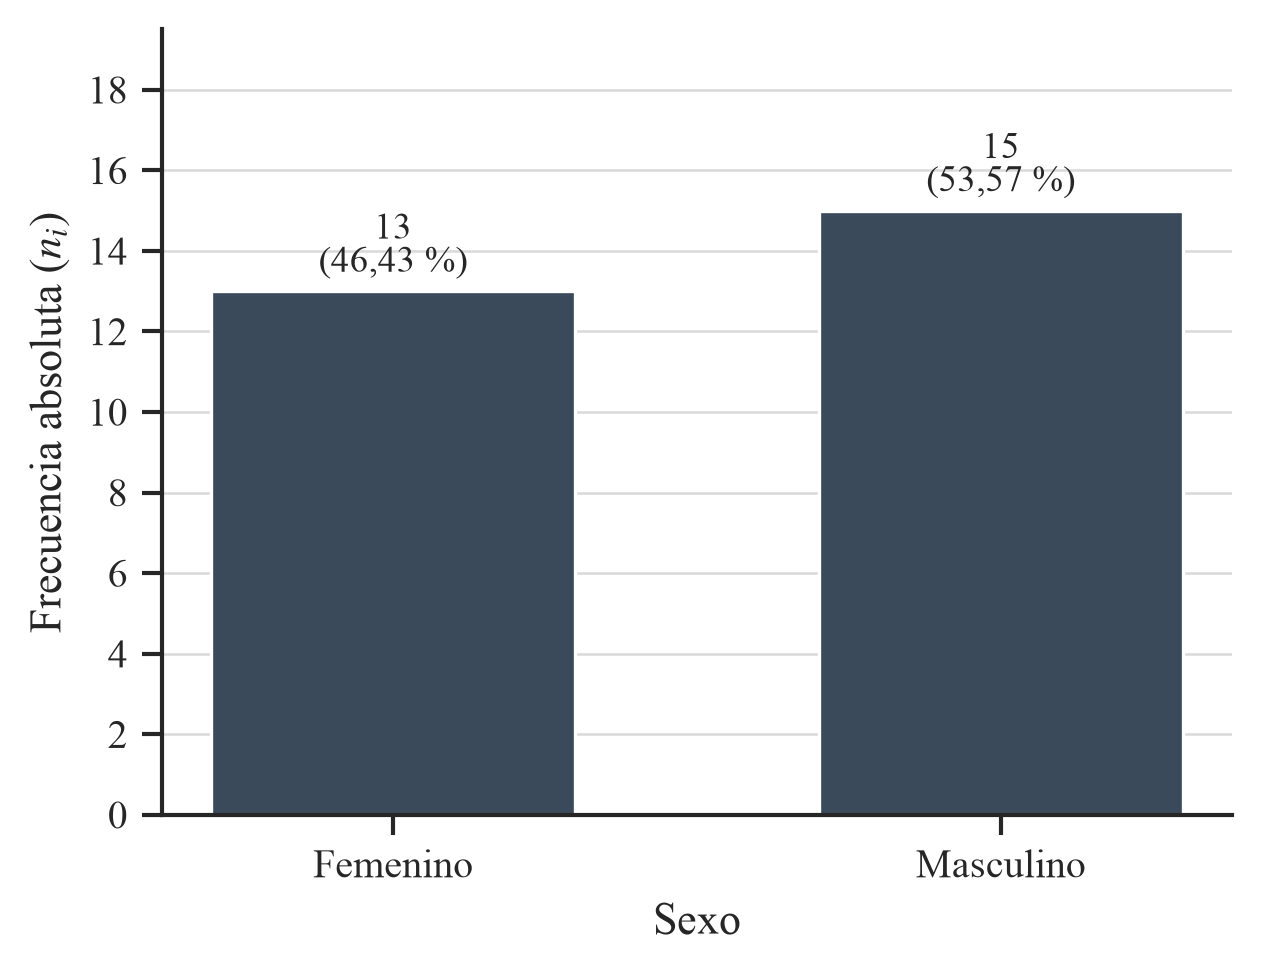
\includegraphics[width=0.72\linewidth, height=0.33\textheight, keepaspectratio]{grafico_sexo.png}
    \caption{Distribución de estudiantes según sexo biológico}
    \label{fig:sexo}
    \fuentefig
\end{figure}

\begin{figure}[H]
    \centering
    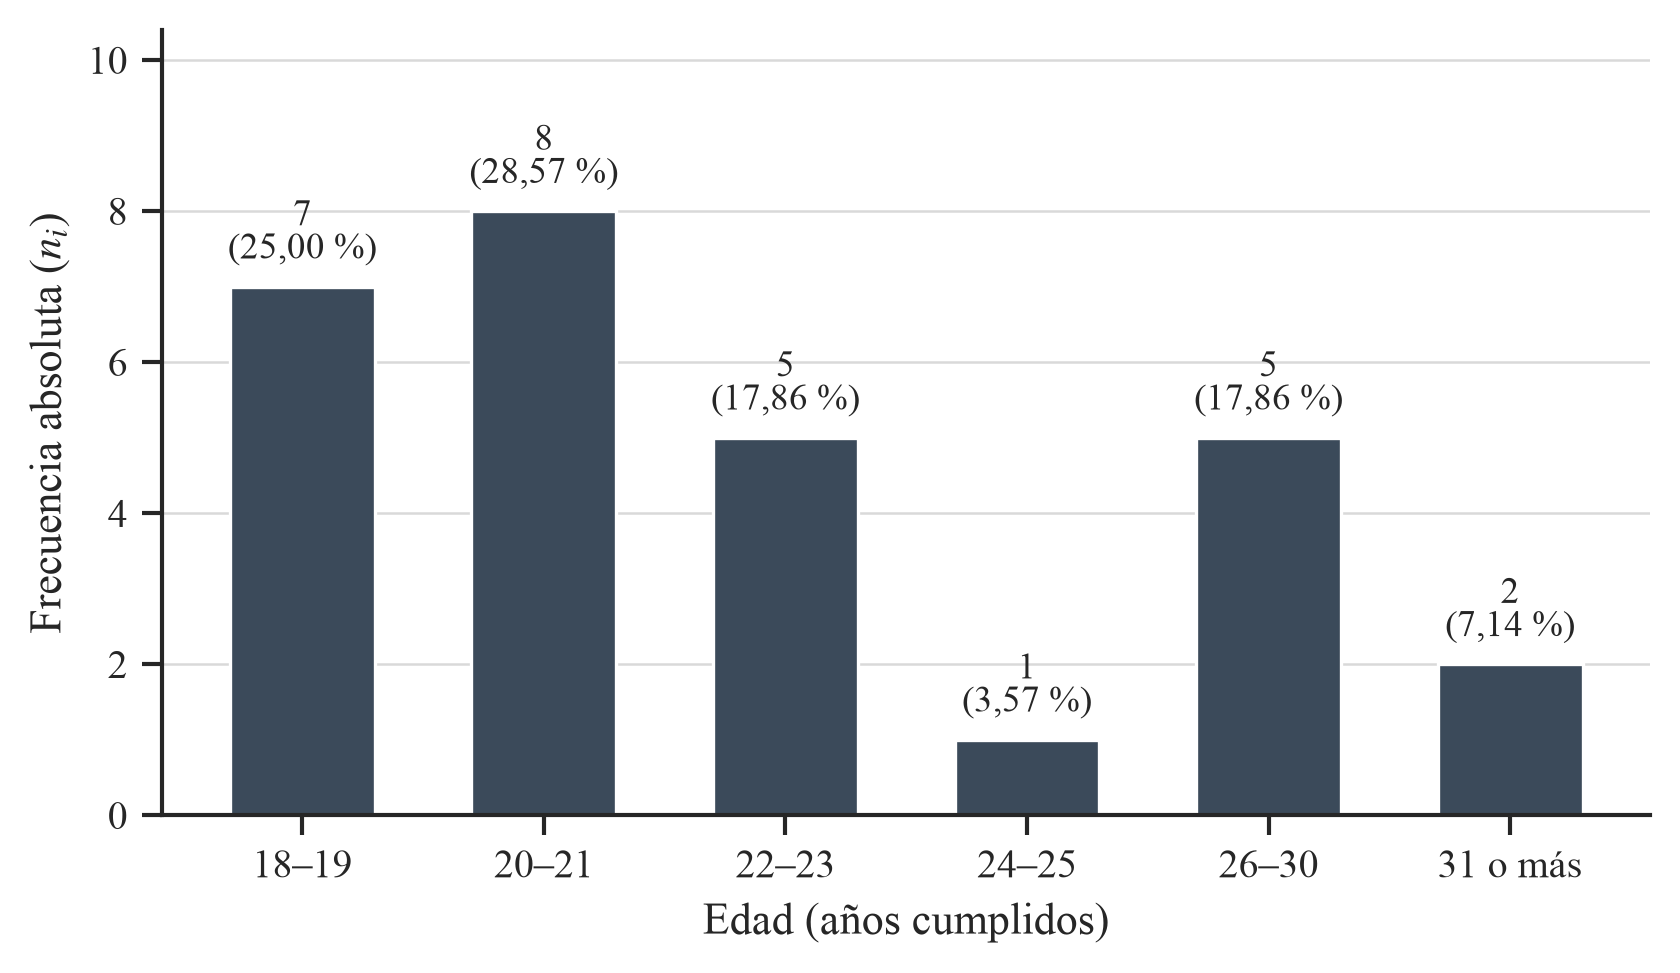
\includegraphics[width=0.84\linewidth, height=0.33\textheight, keepaspectratio]{grafico_edad.png}
    \caption{Distribución de estudiantes según edad cumplida}
    \label{fig:edad}
    \fuentefig
\end{figure}

\begin{figure}[H]
    \centering
    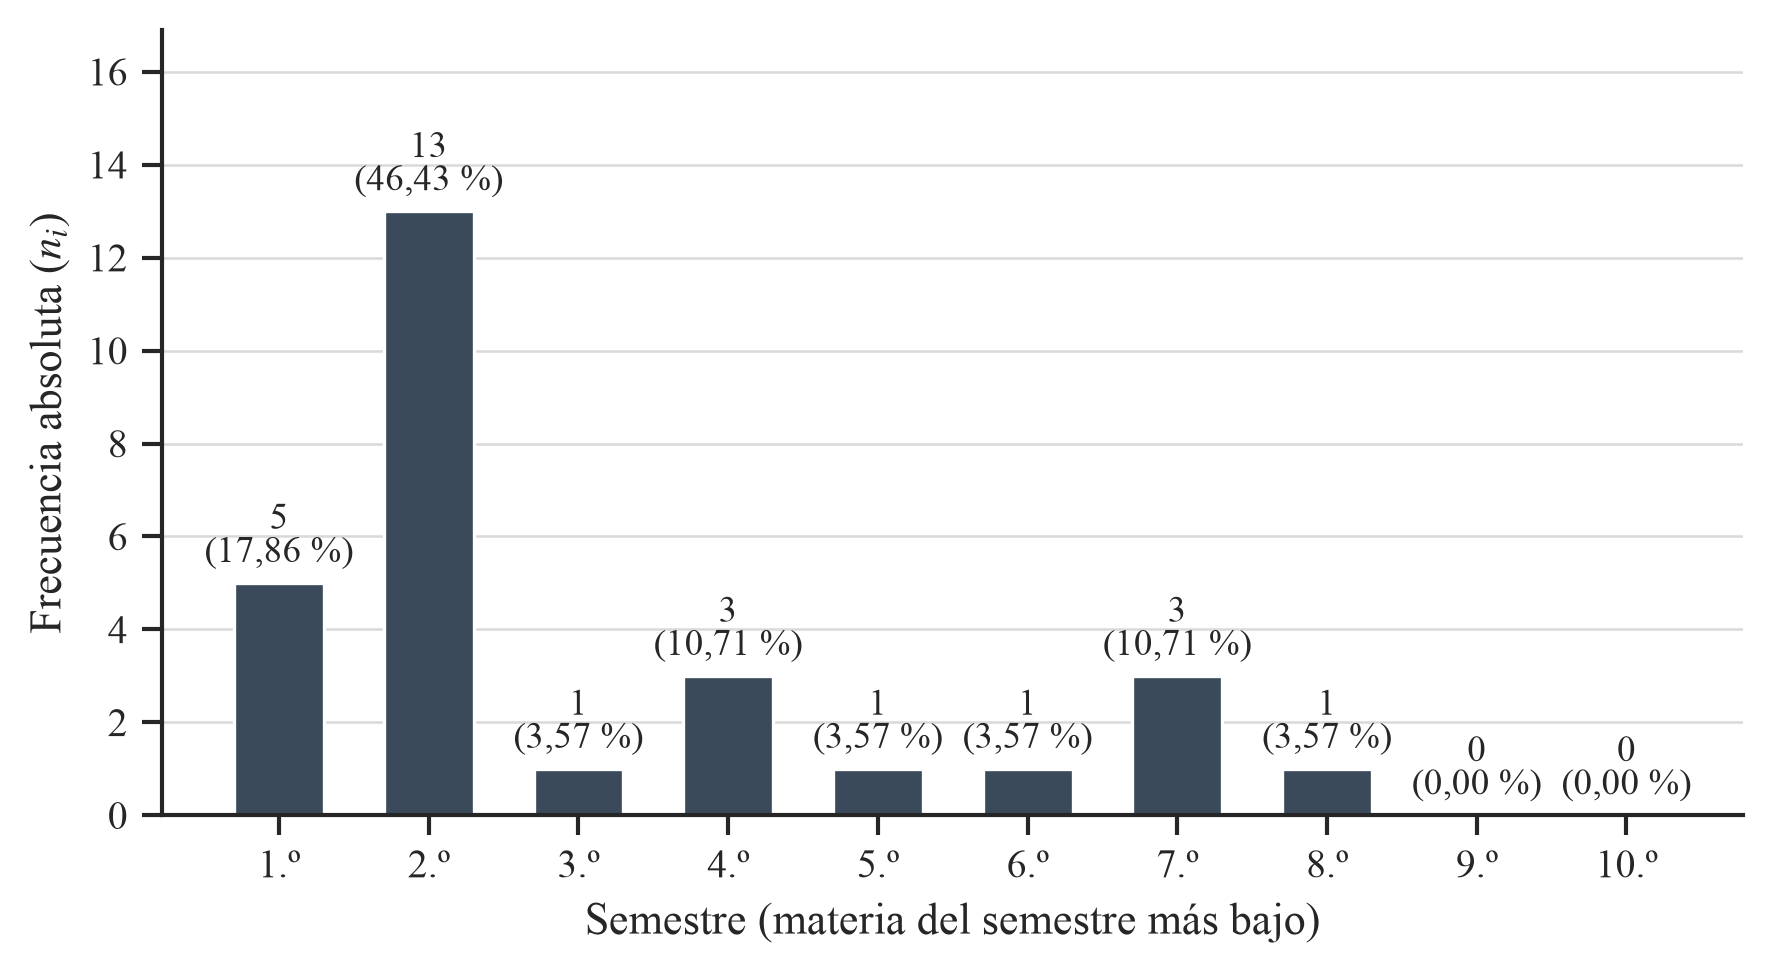
\includegraphics[width=0.88\linewidth, height=0.33\textheight, keepaspectratio]{grafico_semestre.png}
    \caption{Distribución de estudiantes según semestre cursado, materia del semestre más bajo}
    \label{fig:semestre}
    \fuentefig
\end{figure}

\begin{figure}[H]
    \centering
    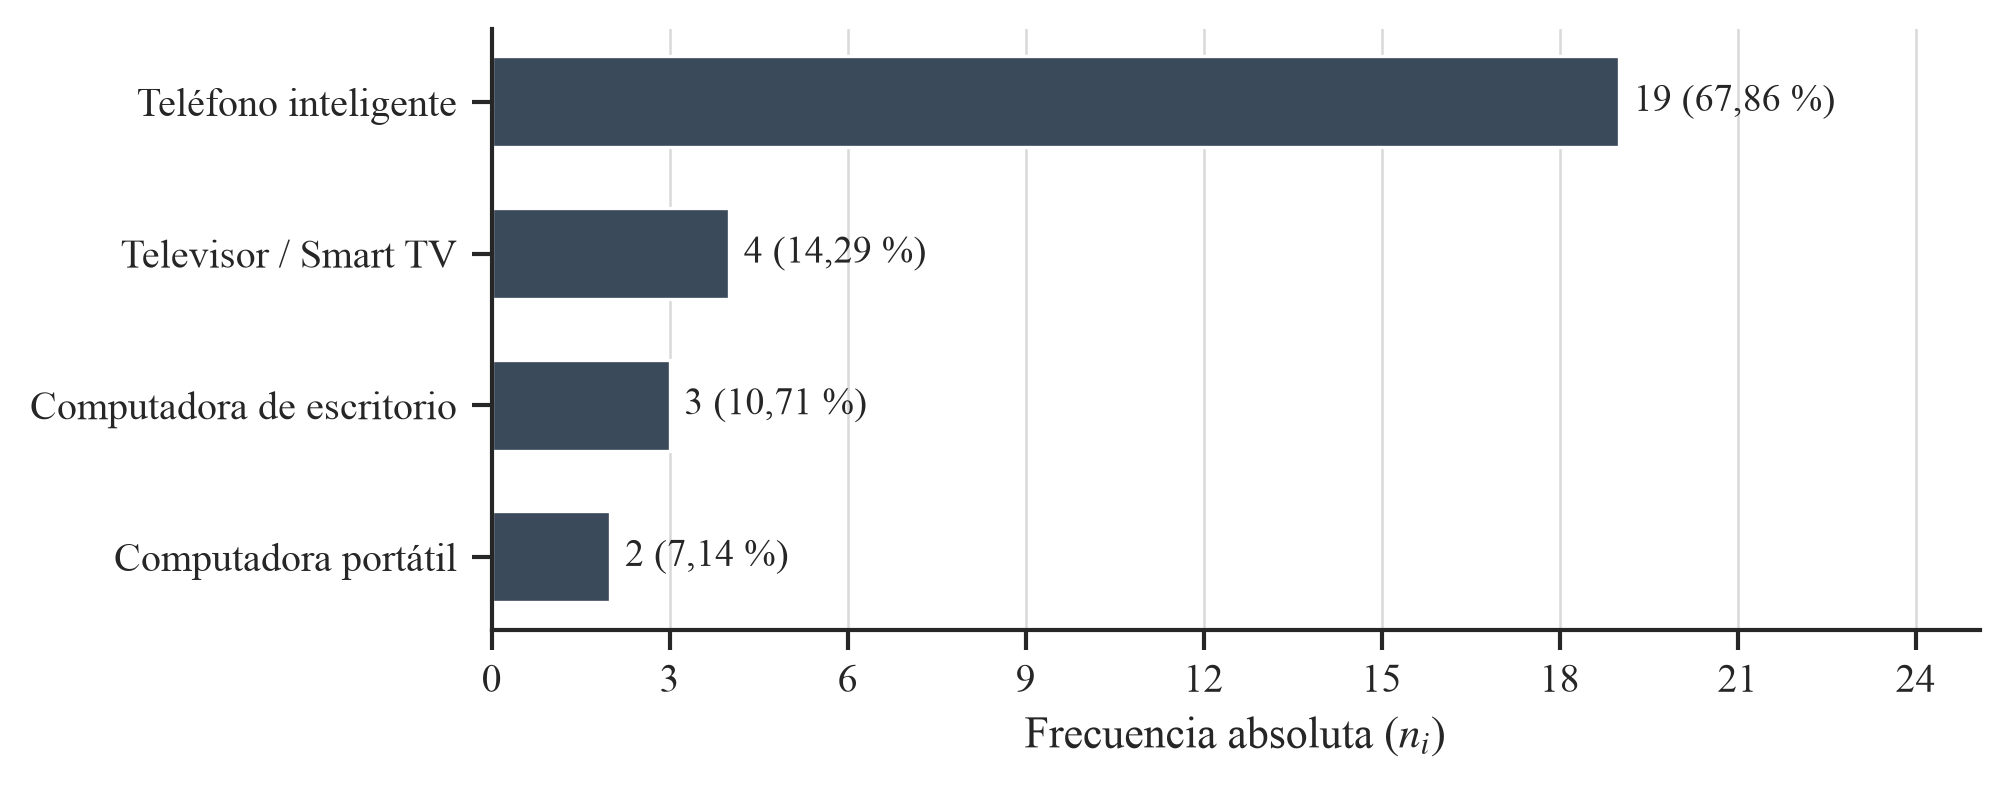
\includegraphics[width=0.86\linewidth, height=0.30\textheight, keepaspectratio]{grafico_dispositivo.png}
    \caption{Distribución según dispositivo principal utilizado antes de dormir}
    \label{fig:dispositivo}
    \fuentefig
\end{figure}

\begin{figure}[H]
    \centering
    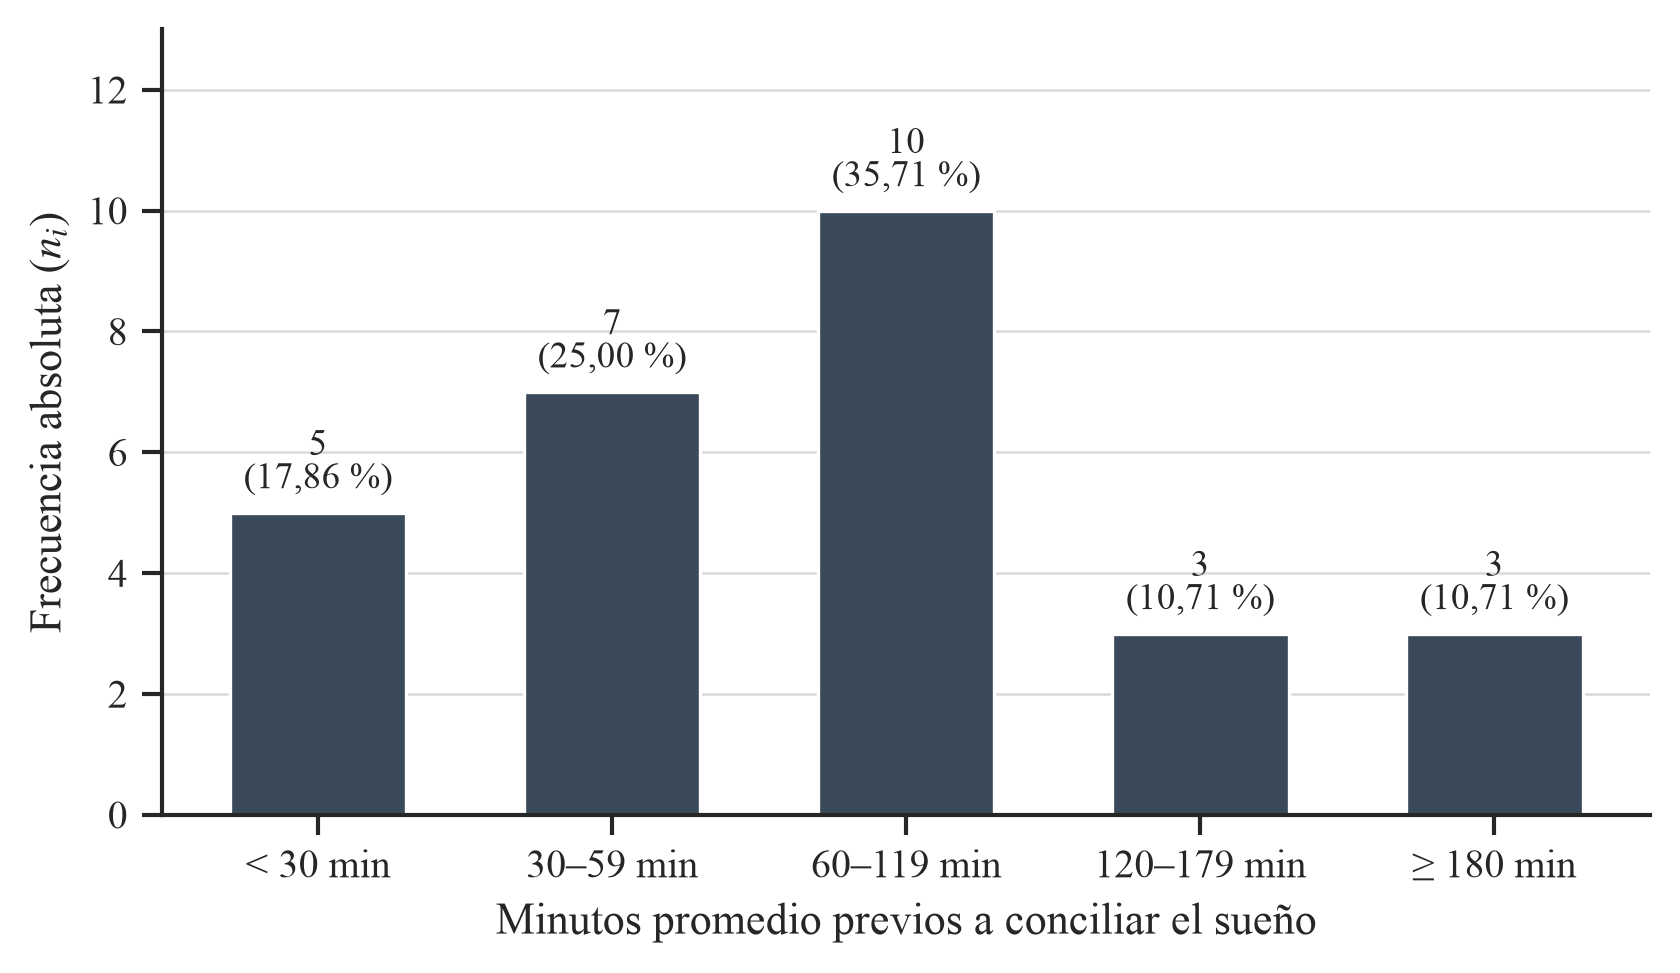
\includegraphics[width=0.84\linewidth, height=0.33\textheight, keepaspectratio]{grafico_tiempo_pantalla.png}
    \caption{Distribución según tiempo promedio de uso nocturno de pantallas antes de dormir}
    \label{fig:tiempo_pantalla}
    \fuentefig
\end{figure}

\begin{figure}[H]
    \centering
    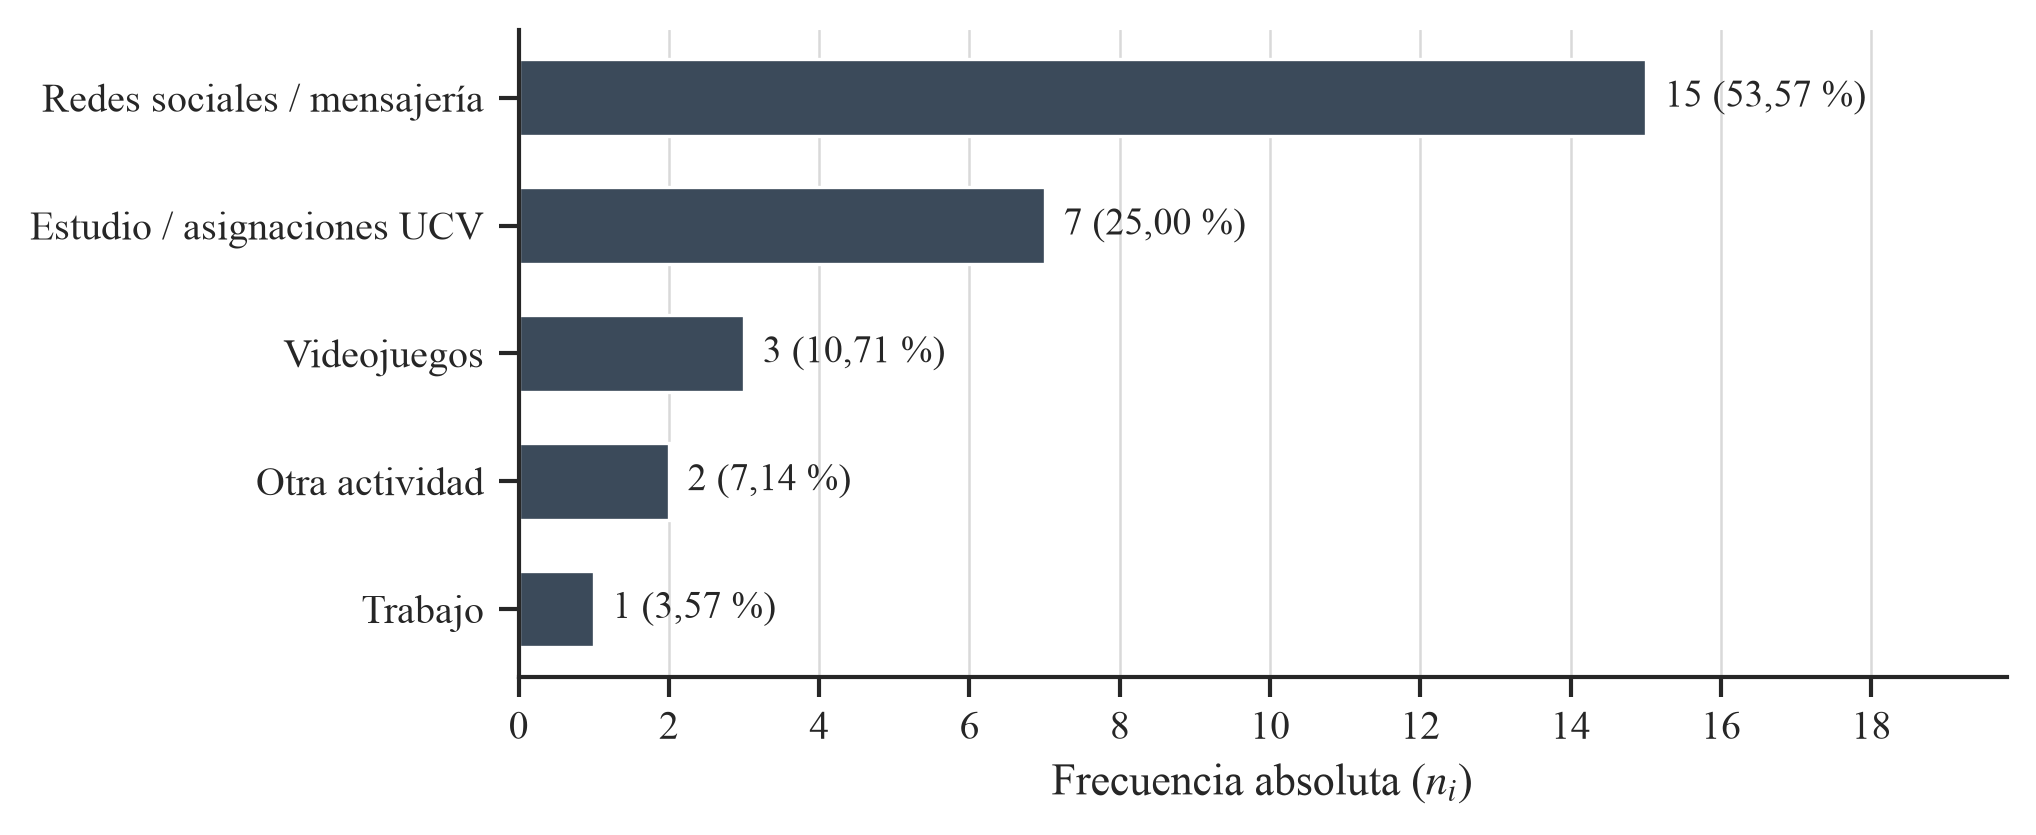
\includegraphics[width=0.86\linewidth, height=0.31\textheight, keepaspectratio]{grafico_actividad.png}
    \caption{Distribución según actividad digital predominante antes de dormir}
    \label{fig:actividad}
    \fuentefig
\end{figure}

\begin{figure}[H]
    \centering
    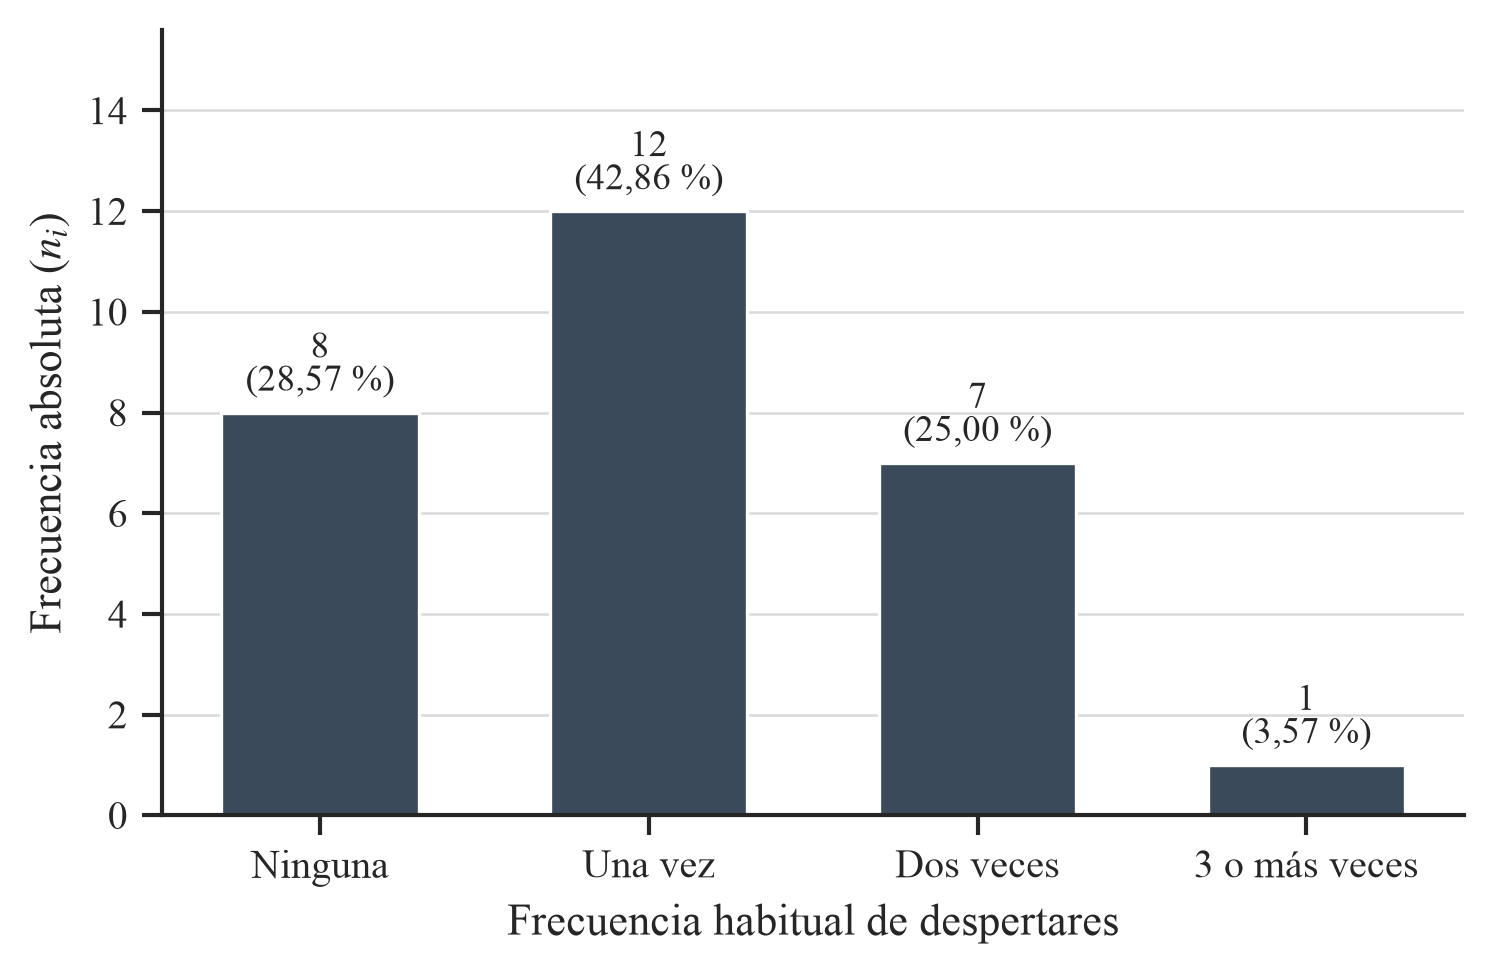
\includegraphics[width=0.80\linewidth, height=0.33\textheight, keepaspectratio]{grafico_despertares.png}
    \caption{Distribución de despertares involuntarios durante la noche}
    \label{fig:despertares}
    \fuentefig
\end{figure}

\begin{figure}[H]
    \centering
    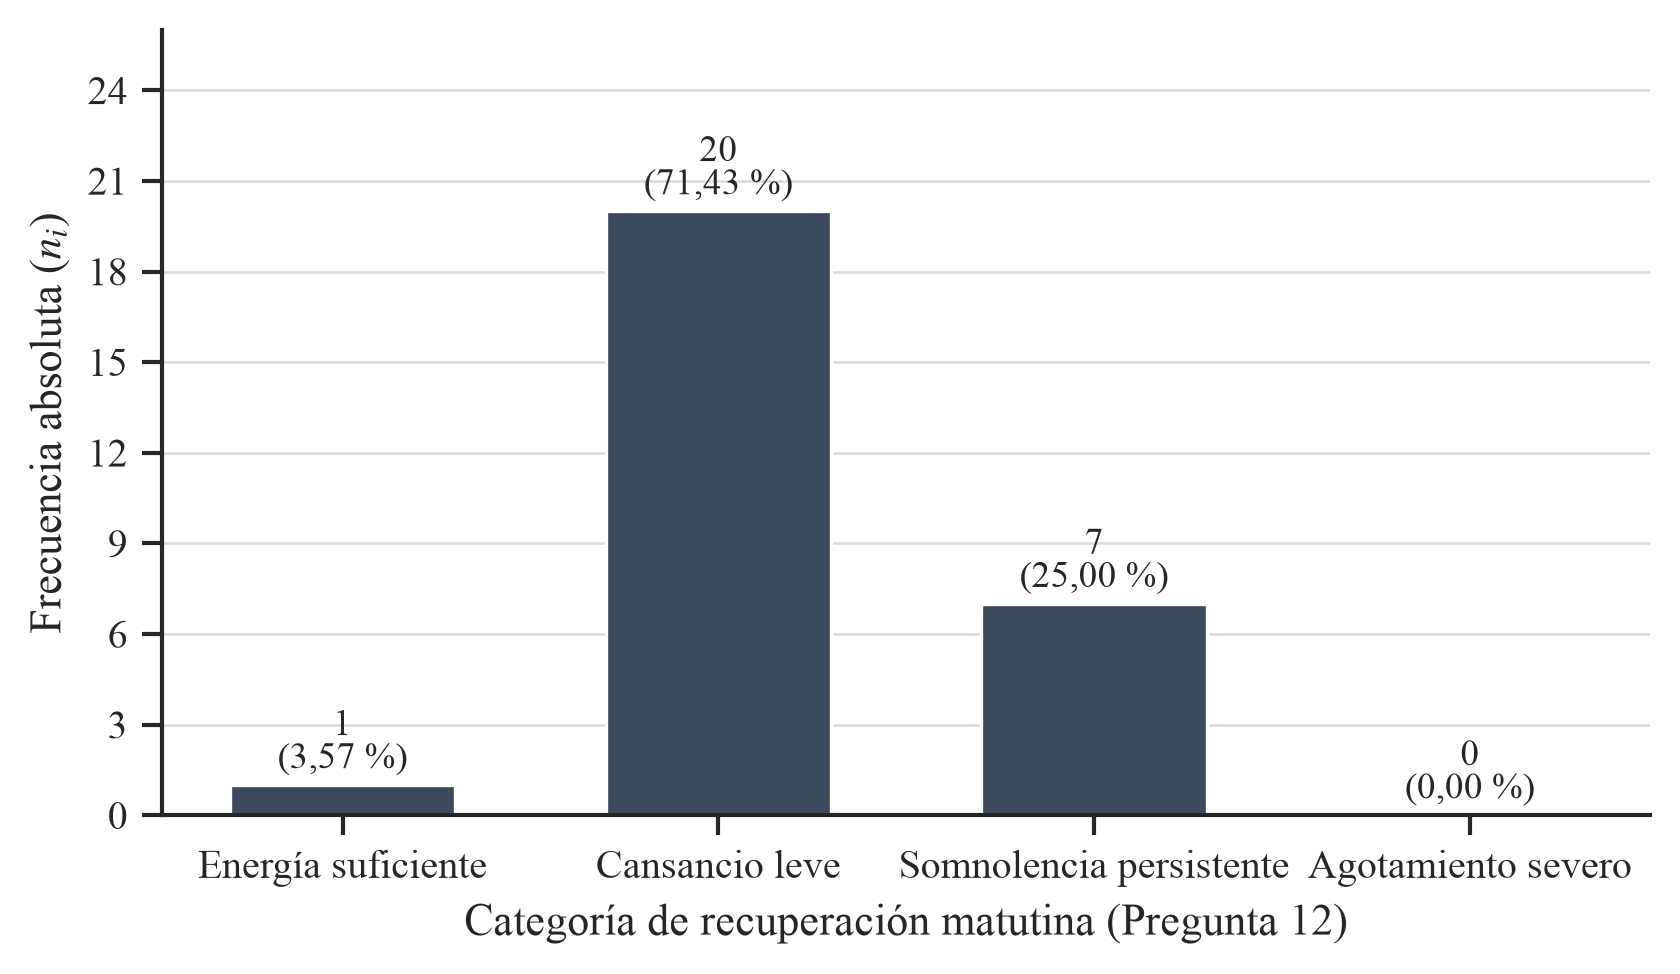
\includegraphics[width=0.84\linewidth, height=0.33\textheight, keepaspectratio]{grafico_sensacion.png}
    \caption{Distribución de la sensación habitual al despertar en las mañanas}
    \label{fig:sensacion}
    \fuentefig
\end{figure}

\begin{figure}[H]
    \centering
    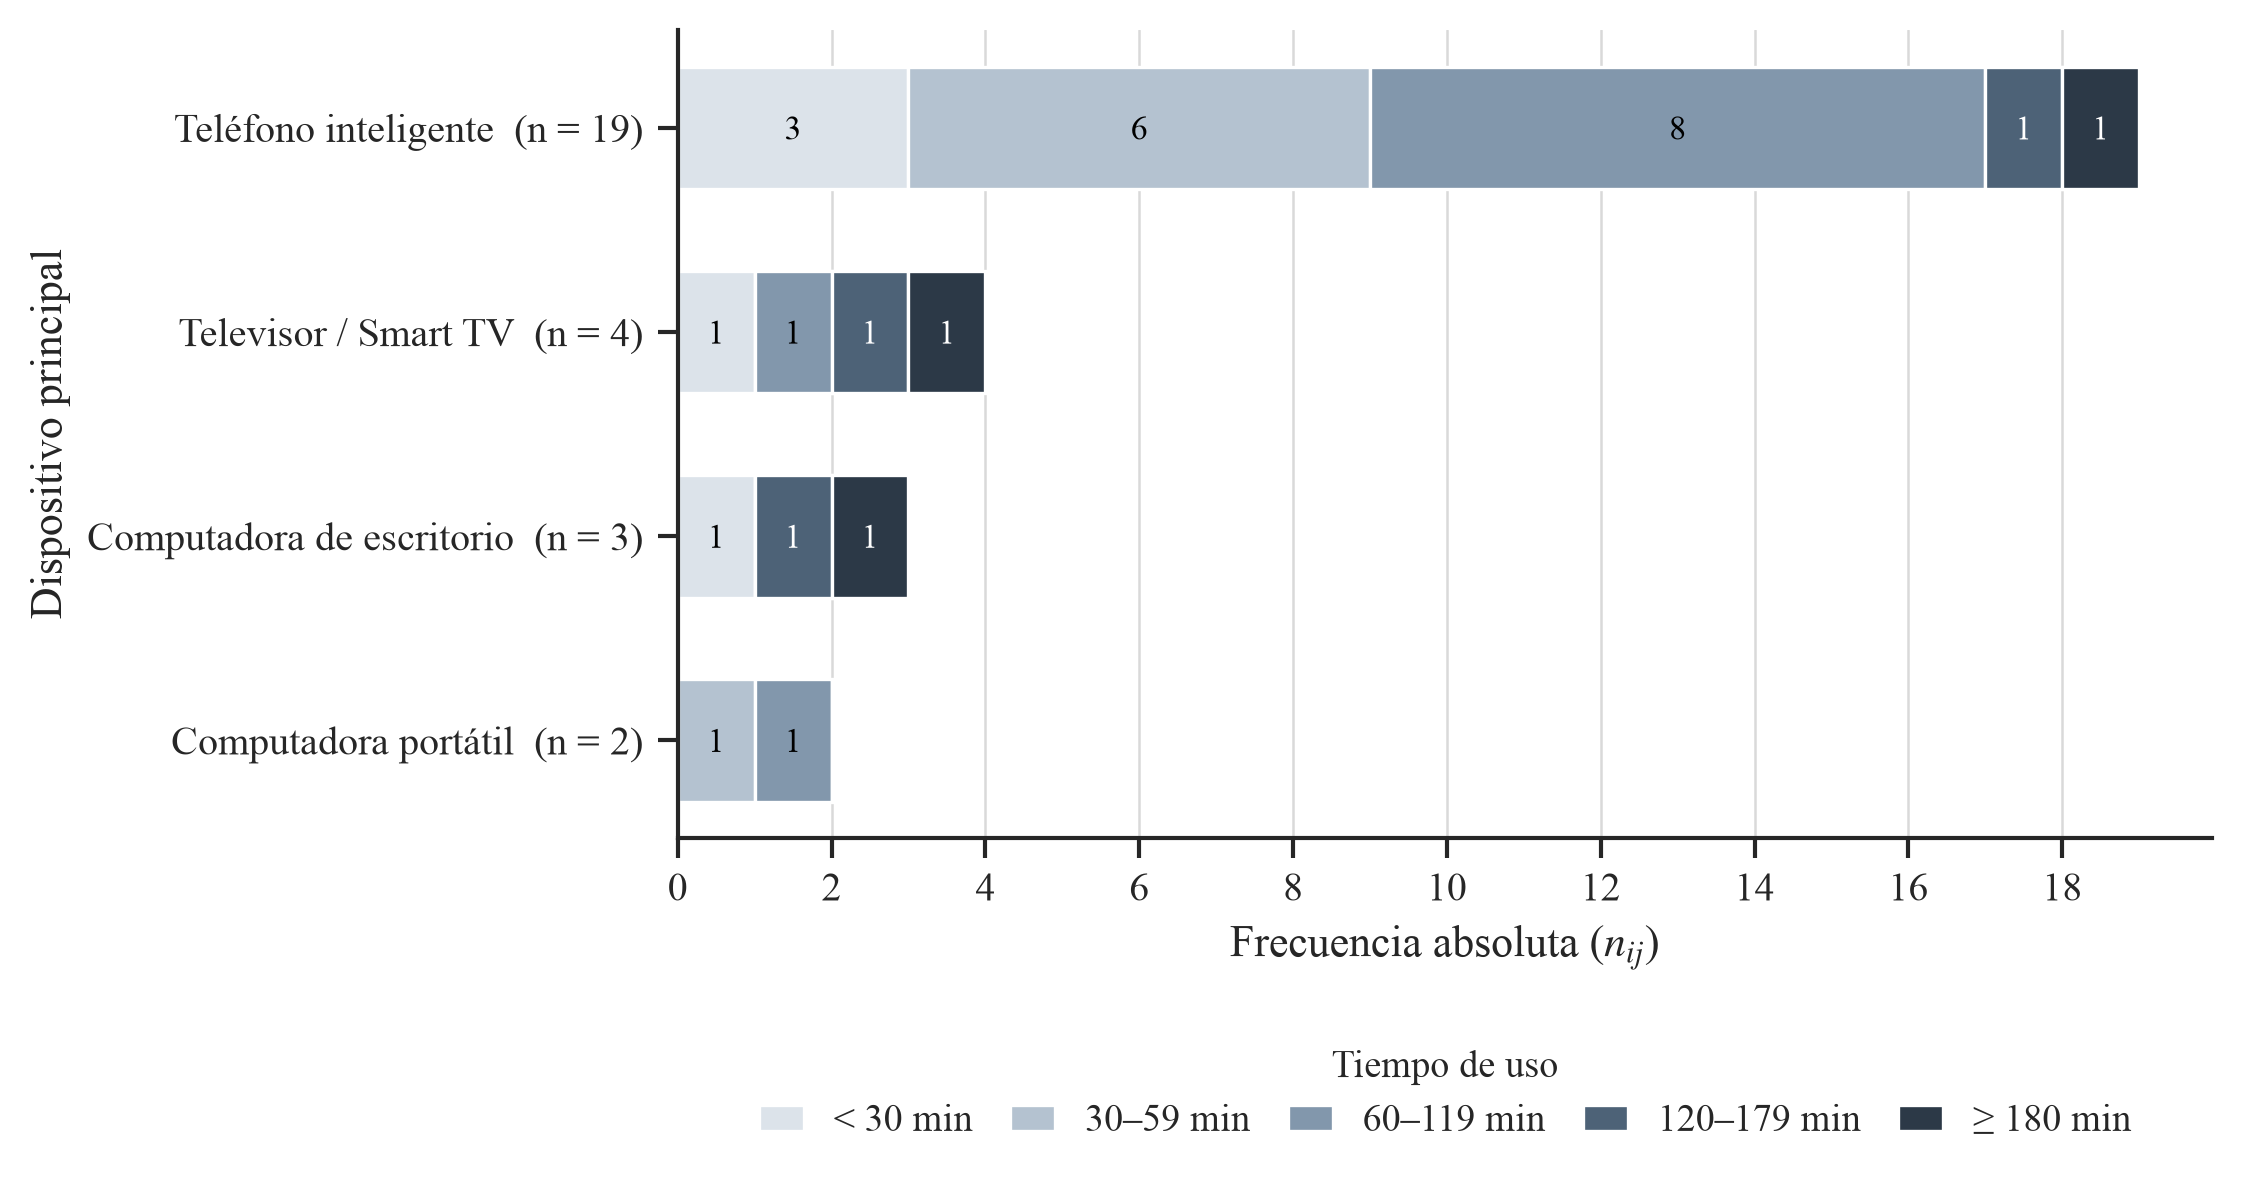
\includegraphics[width=0.90\linewidth, height=0.38\textheight, keepaspectratio]{grafico_dispositivo_tiempo.png}
    \caption{Dispositivo principal utilizado según tramo de tiempo de uso nocturno}
    \label{fig:dispositivo_tiempo}
    \fuentefig
\end{figure}

\begin{figure}[H]
    \centering
    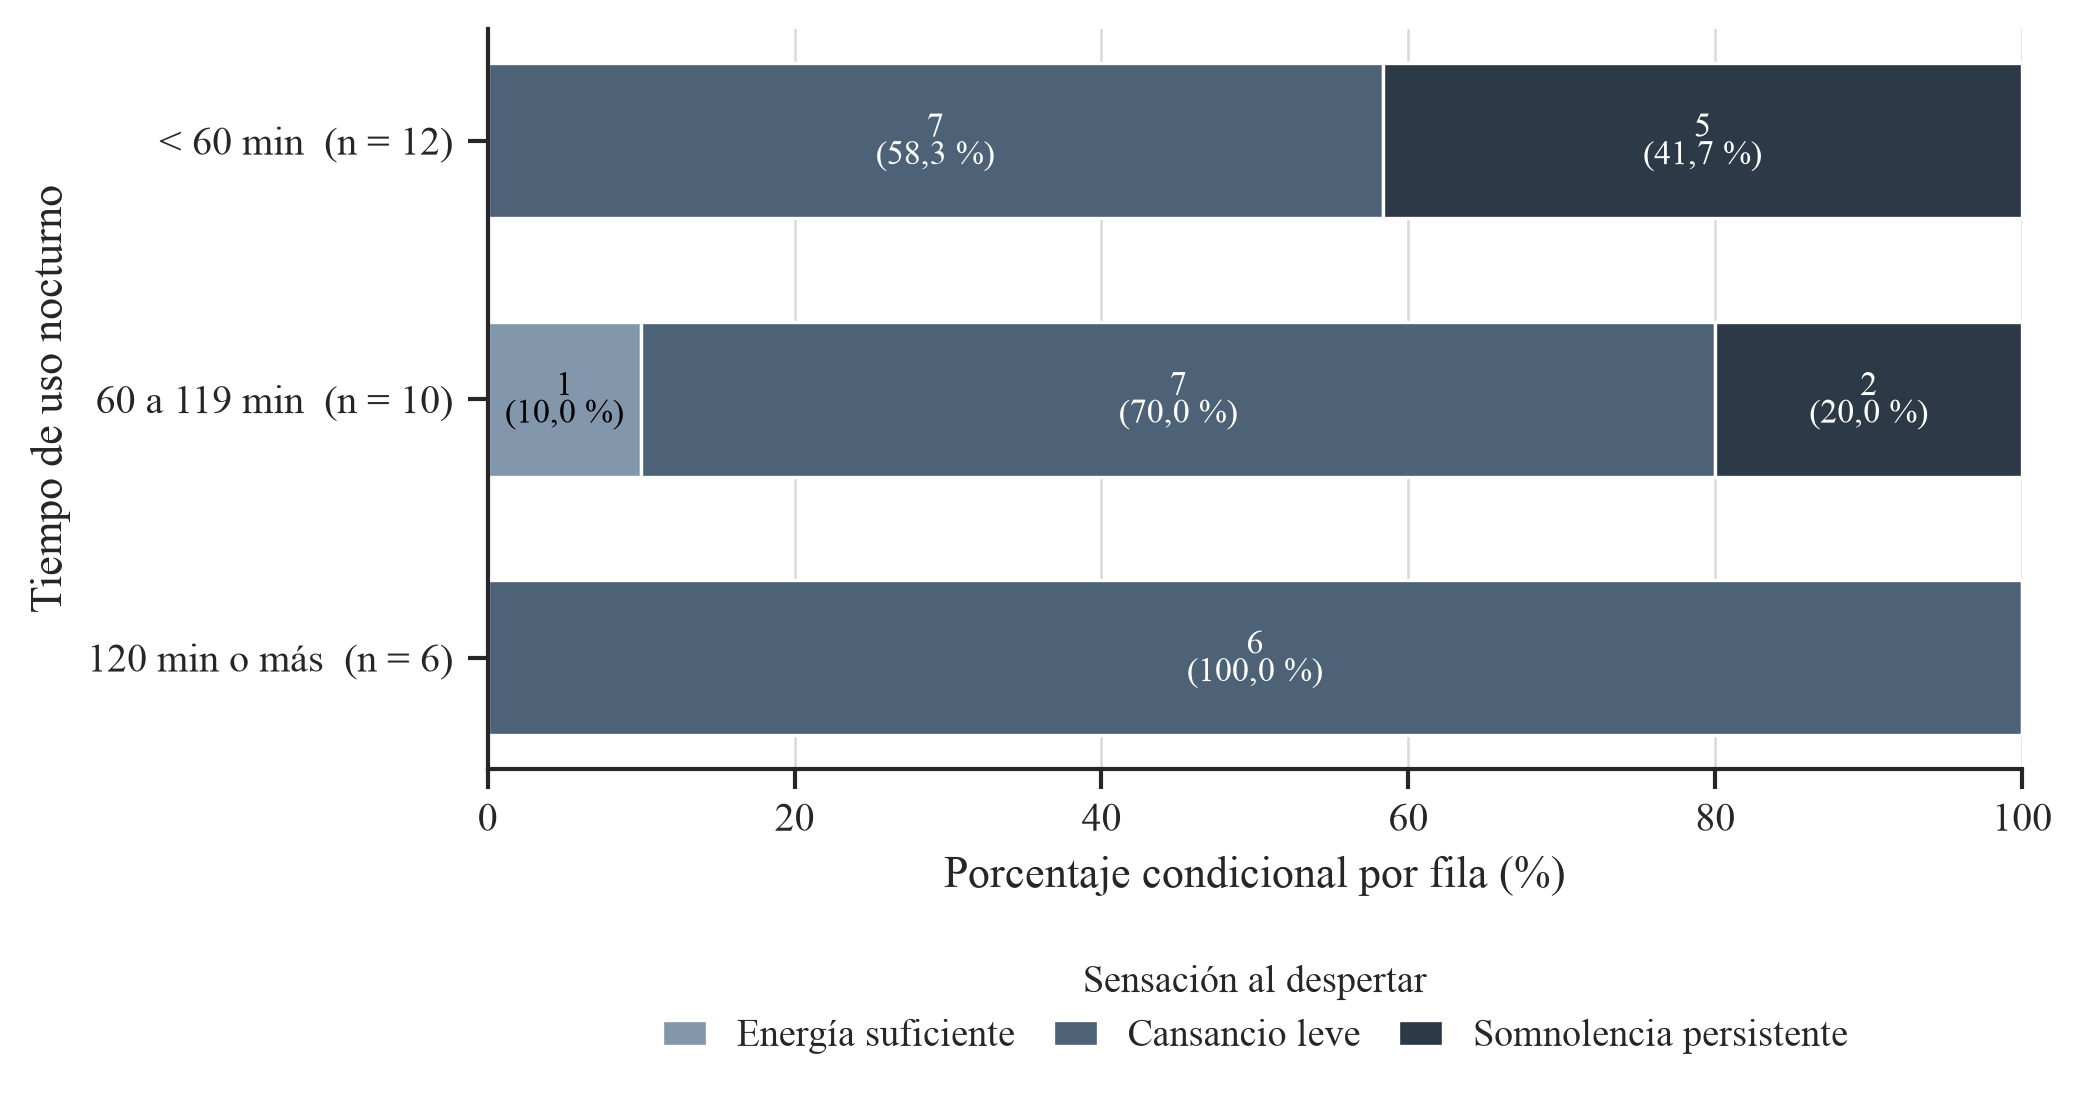
\includegraphics[width=0.90\linewidth, height=0.35\textheight, keepaspectratio]{grafico_tiempo_calidad.png}
    \caption{Distribución porcentual condicional de la sensación habitual al despertar según tiempo de pantalla}
    \label{fig:tiempo_calidad}
    \fuentefig
\end{figure}

\begin{figure}[H]
    \centering
    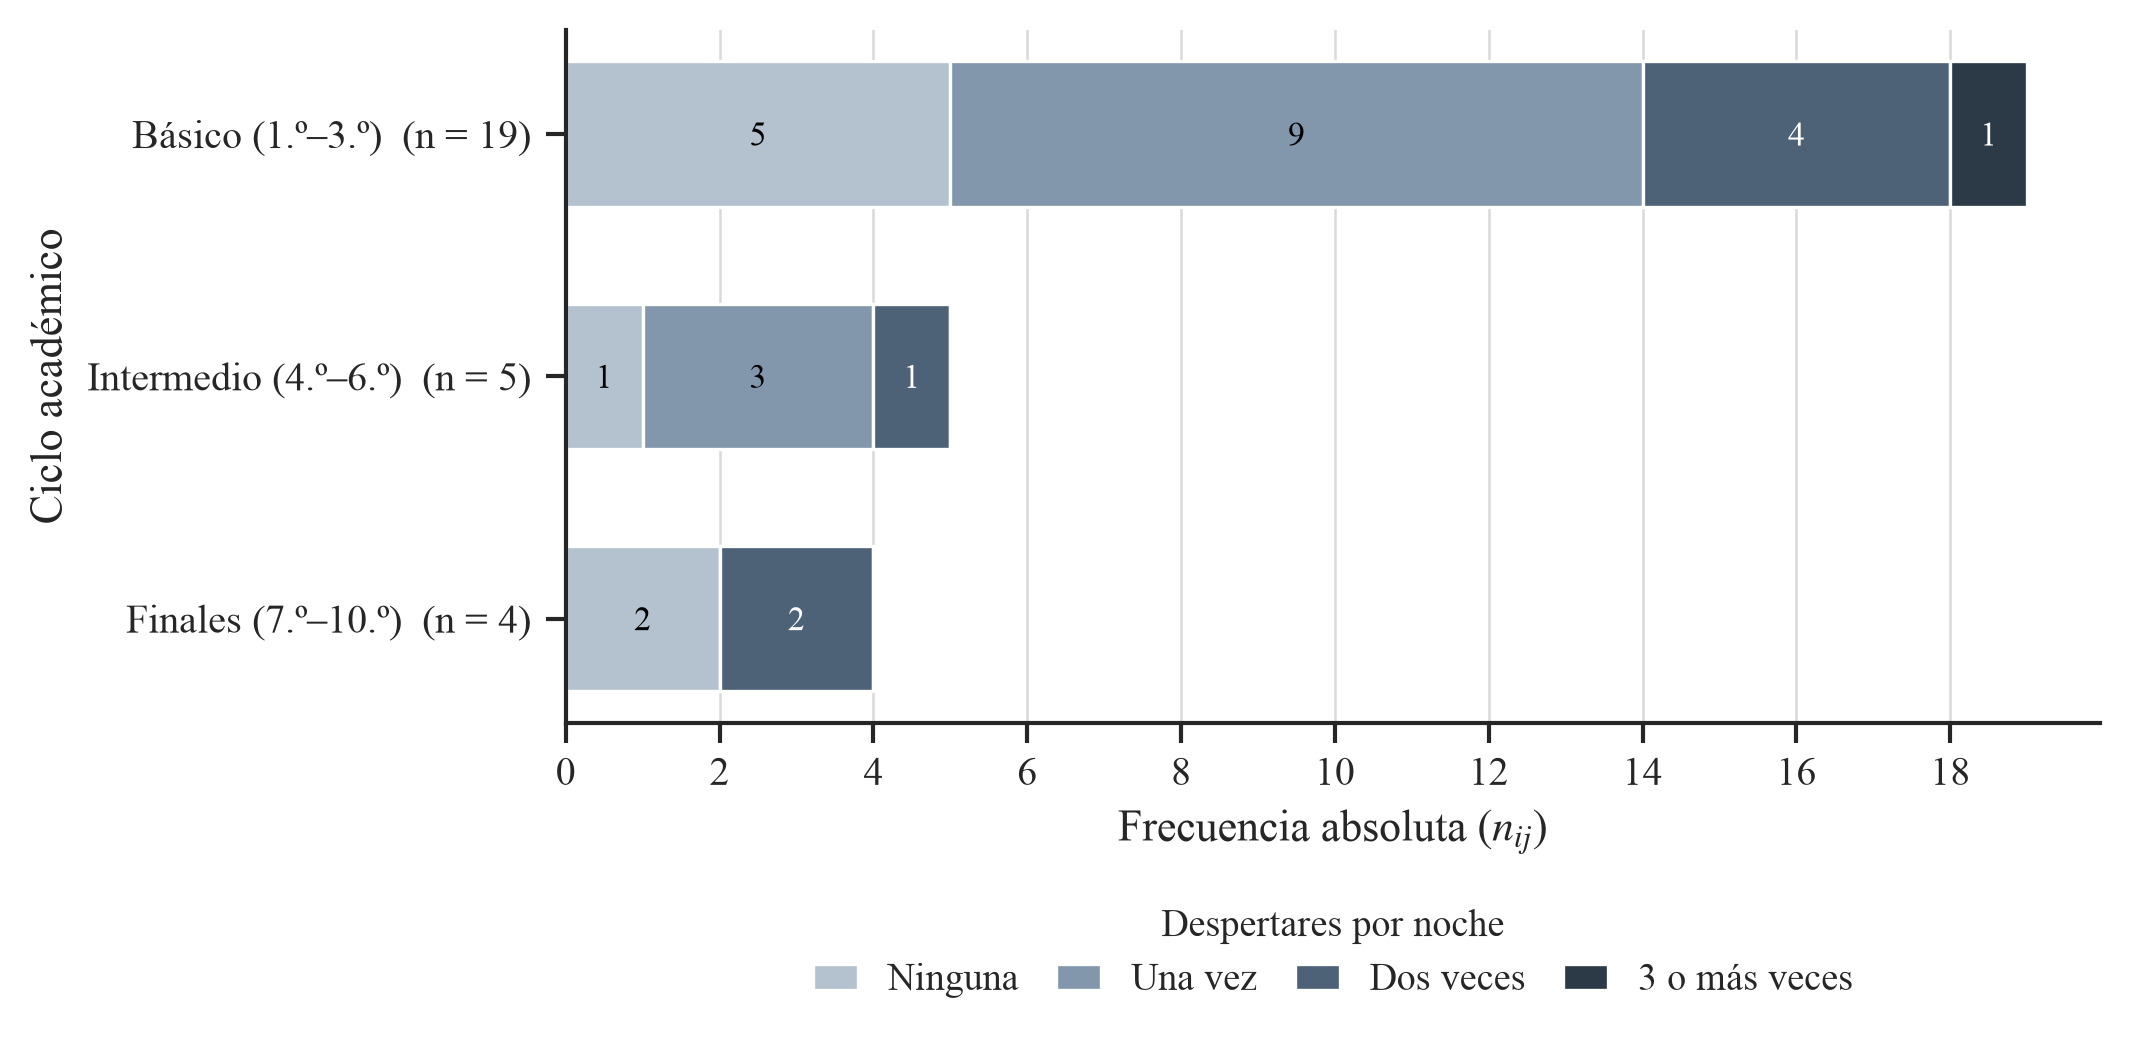
\includegraphics[width=0.90\linewidth, height=0.35\textheight, keepaspectratio]{grafico_ciclo_despertares.png}
    \caption{Frecuencia de despertares nocturnos involuntarios según ciclo académico}
    \label{fig:ciclo_despertares}
    \fuentefig
\end{figure}

\subsubsection{Gráficos Analíticos e Inferenciales \texorpdfstring{($n = 28$)}{(n = 28)}}

\begin{figure}[H]
    \centering
    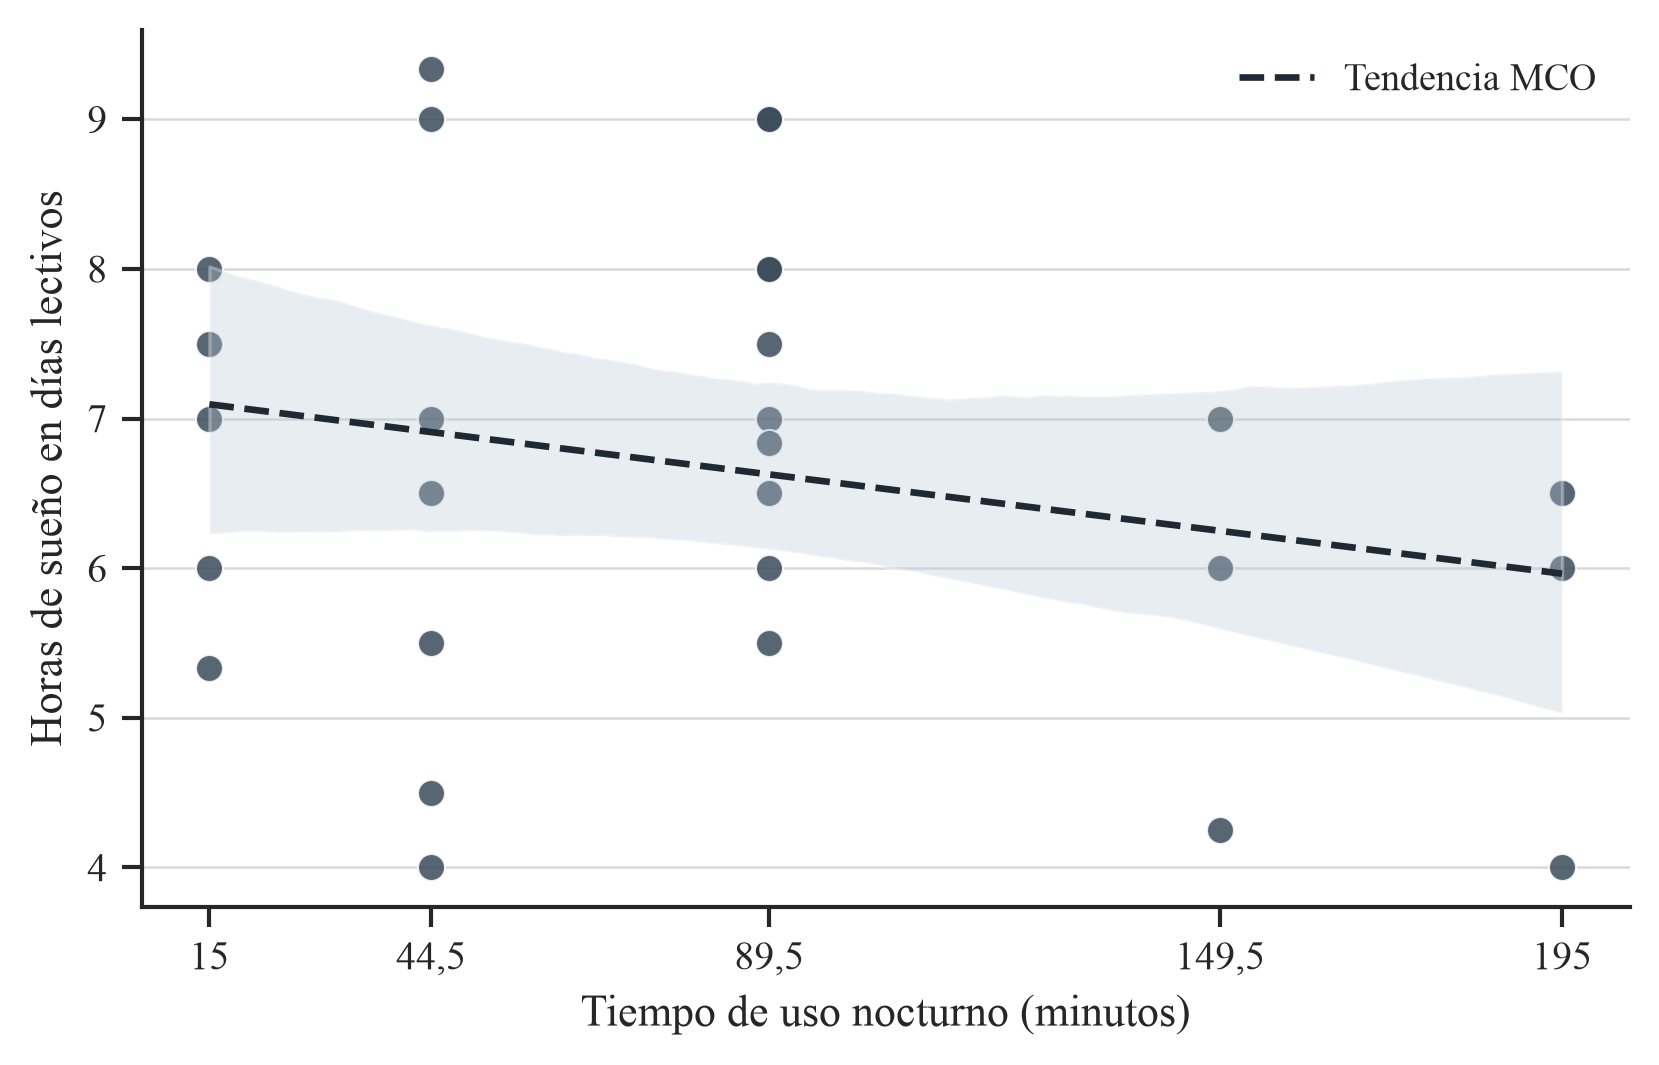
\includegraphics[width=0.86\linewidth, height=0.37\textheight, keepaspectratio]{grafico1_dispersion.png}
    \caption{Diagrama de dispersión y recta de tendencia MCO entre tiempo de uso nocturno y horas estimadas de sueño en días lectivos}
    \label{fig:dispersion}
    \fuentefig
\end{figure}

\begin{figure}[H]
    \centering
    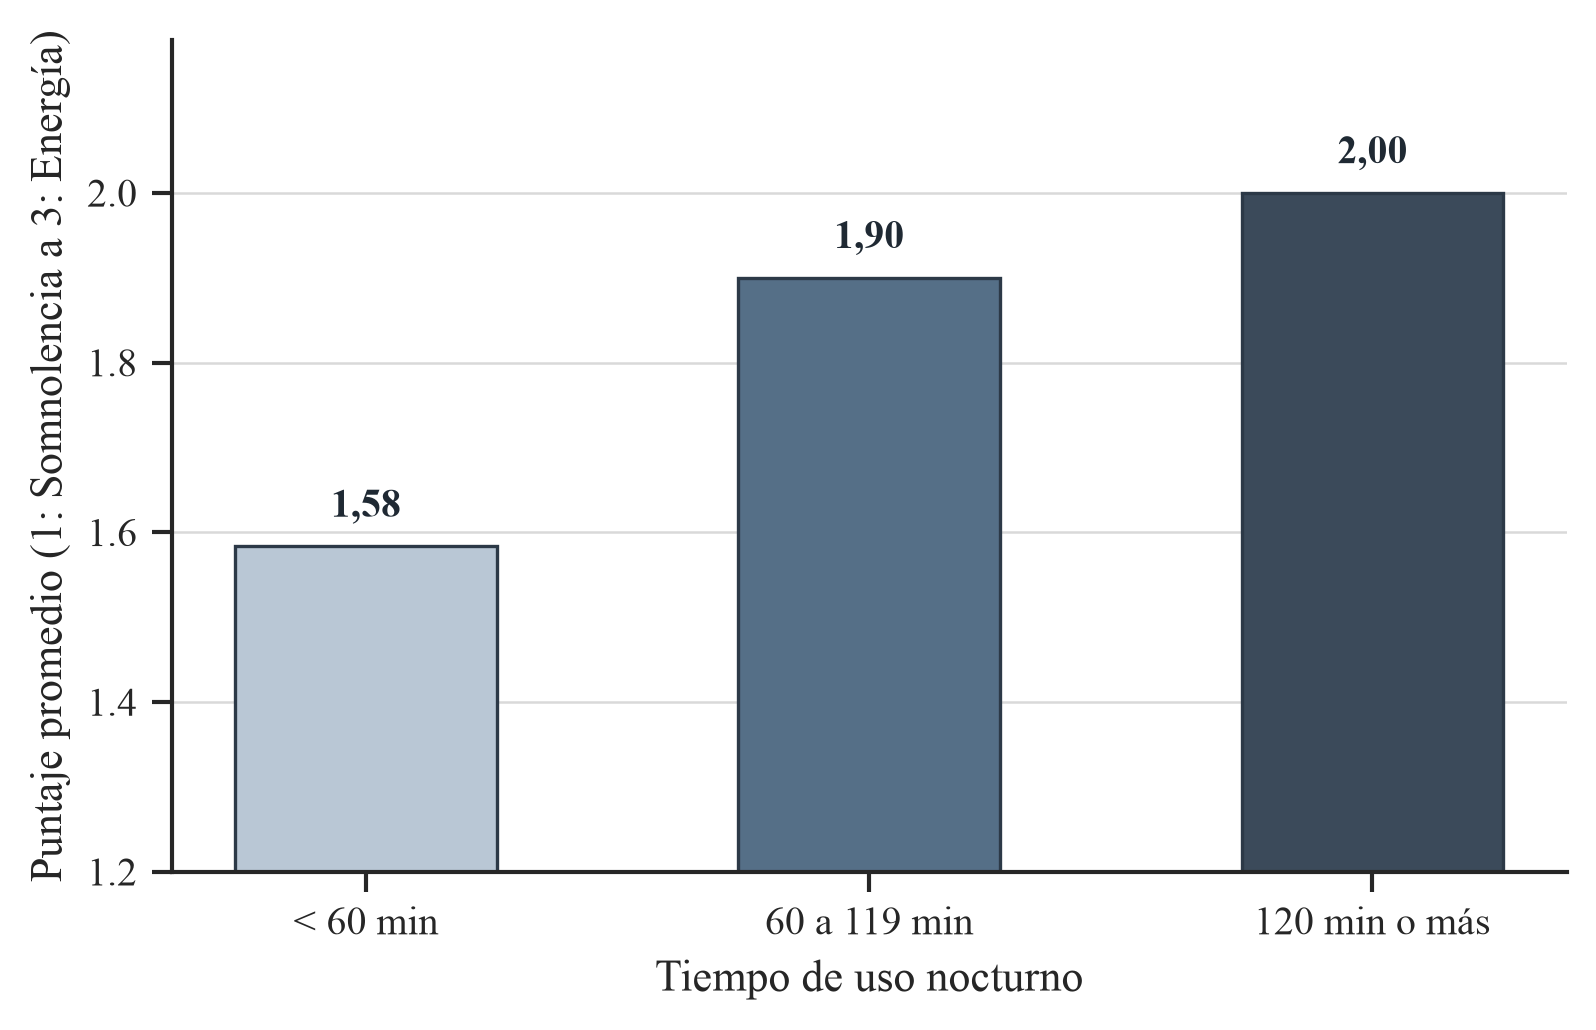
\includegraphics[width=0.86\linewidth, height=0.37\textheight, keepaspectratio]{grafico2_calidad_pantallas.png}
    \caption{Puntaje promedio de sensación al despertar, escala 1: somnolencia a 3: energía, según tramo de exposición a pantallas}
    \label{fig:calidad}
    \fuentefig
\end{figure}

\begin{figure}[H]
    \centering
    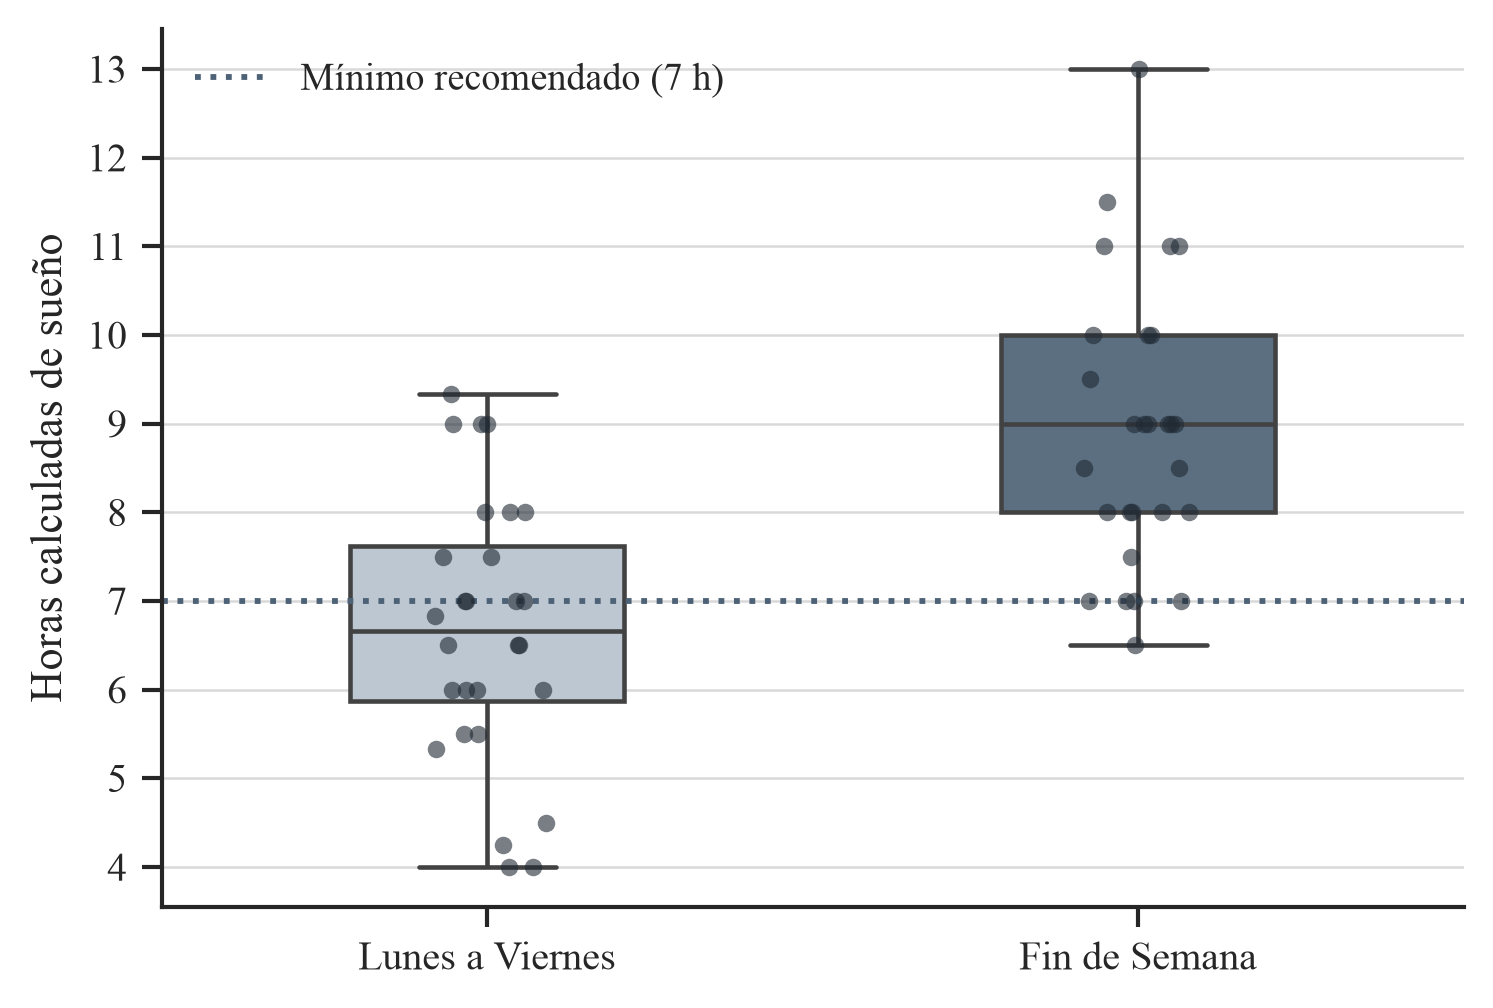
\includegraphics[width=0.80\linewidth, height=0.37\textheight, keepaspectratio]{grafico3_semana_vs_finde.png}
    \caption{Distribución comparativa de las horas calculadas de sueño en días lectivos frente a fines de semana}
    \label{fig:cajas}
    \fuentefig
\end{figure}


\subsection{Interpretación y Análisis de Resultados}

Los datos de los 28 estudiantes muestran tres resultados principales:

\begin{enumerate}
    \item \textbf{Prevalencia de dispositivos y tiempo de exposición:}
    En el Cuadro~\ref{tab:c1} se observa que el 67,86\,\% de los estudiantes de la Escuela utilizan teléfonos inteligentes horas previas al descanso. Esto tiene mayor peso fisiológico porque el teléfono suele mirarse a unos 20 o 30 centímetros de la cara, lo que aumenta la entrada directa de luz en la retina y frena la melatonina mucho más que un televisor, usado solo por el 14,29\,\%.

    El Cuadro~\ref{tab:c2} demuestra que el 57,14\,\% de los estudiantes supera los 60 minutos de uso continuo de dispositivos electrónicos horas previas al descanso, lo cual abre una ventana a la estimulación lumínica producida por la luz azul, generando sobreestimulación cognitiva en horas previas al reposo.

    \item \textbf{Déficit lectivo y compensaciones en fines de semana:}
    El Cuadro~\ref{tab:c3} y el Cuadro~\ref{tab:c4} presentados anteriormente exponen que el 53,57\,\% de los estudiantes que respondieron la encuesta se privan del sueño durante los días de mayor actividad académica, de lunes a viernes, en los cuales duermen menos de 7 horas. Se puede observar que de hecho los estudiantes promedian 6,67 horas de descanso durante estos días de semana.

    Por el contrario, durante los fines de semana los estudiantes suelen expandir en promedio su descanso compensando ese déficit generado en la semana laboral. En fines de semana estos estudiantes registraron un promedio de 8,93 horas de descanso, lo cual compensa 2,26 horas adicionales a las que dormirían en promedio en días laborales. Este patrón revelado en la muestra expone el denominado comportamiento de \textit{Jetlag Social}, donde el estudiante acumula una deuda de sueño semanal impuesta por los compromisos académicos y laborales y la intenta compensar en los días libres.

    \item \textbf{Disociación cuantitativa y cualitativa:}
    La estimación del modelo de regresión lineal expuesta en el Cuadro~\ref{tab:c7} y en el Gráfico~\ref{fig:dispersion} revela que la pendiente entre los minutos de exposición a las pantallas y la duración del sueño no alcanzó la significancia requerida. Sin embargo, si observamos la correlación de Spearman en el Cuadro~\ref{tab:c8} y en el Gráfico~\ref{fig:calidad}, se constata que arrojó una correlación positiva y estadísticamente significativa con la sensación matutina al despertar. Este hallazgo muestra que la exposición a las pantallas de dispositivos electrónicos en los estudiantes no reduce el tiempo de descanso en la cama de forma lineal, ya que la hora de despertar de los estudiantes es una variable exógena regida por el horario académico, mientras el puntaje promedio en la escala subjetiva del Cuadro~\ref{tab:c5} pasa de 1,58 puntos a 2,00 puntos en exposiciones prolongadas sin mostrar deterioro matutino en esta muestra.
\end{enumerate}


\subsection{Inferencias}

\subsubsection{Estimación por Intervalos}

Con la muestra de 28 estudiantes de la EECA se calcularon intervalos de confianza del 95\,\% para los parámetros clave empleando la distribución $t$ de Student con 27 grados de libertad debido al tamaño reducido de la muestra.

La media del sueño en días lectivos arrojó un intervalo de $\mu_{\text{sem}}$ entre $6{,}08$ y $7{,}26$ horas; el límite inferior muestra que buena parte del grupo duerme cerca de las 6 horas.

La media del sueño en fines de semana arrojó un intervalo de $\mu_{\text{fin}}$ entre $8{,}32$ horas y $9{,}54$ horas, el cual no presenta intersección con el intervalo anterior en los días de semana lectiva; como ambos promedios provienen de los mismos 28 estudiantes, el cambio real se evalúa con el intervalo de la diferencia individual $\Delta t$.

La media de compensación horaria se encontró en un intervalo de $1{,}42$ horas a $3{,}10$ horas. Al excluir el cero, indica que efectivamente la muestra estudiantil posee una deuda de sueño durante la semana, la cual es compensada los días de fines de semana.

\subsubsection{Contraste de Hipótesis}

Se realizaron 4 pruebas de contraste de hipótesis en esta investigación, resumidas en el Cuadro~\ref{tab:c10} al 5\,\% de significancia, las cuales son expuestas a continuación:

\begin{enumerate}
    \item \textbf{Prueba de Hipótesis 1 correspondiente al déficit de sueño respecto al umbral saludable:}
    $$H_0: \mu_{\text{sem}} \ge 7 \quad \text{vs.} \quad H_1: \mu_{\text{sem}} < 7$$
    Se obtuvo un $t = -1{,}1559$ y $p = 0{,}1289$, por lo que no se rechaza la hipótesis nula. A pesar de que la medida es deficitaria, la variabilidad en la muestra y el tamaño de la misma limitan la potencia del contraste de hipótesis para certificar el déficit generalizado al 95\,\%.

    \item \textbf{Prueba de Hipótesis 2 sobre asimetría semanal y fenómeno del Jetlag Social:}
    $$H_0: \mu_{\Delta t} \le 0 \quad \text{vs.} \quad H_1: \mu_{\Delta t} > 0$$
    La prueba arroja un $t = 5{,}5401$ con $p = 3{,}58 \times 10^{-6}$, por lo que se rechaza la hipótesis nula y existe una compensación horaria real en términos del descanso en los fines de semana.

    \item \textbf{Prueba de Hipótesis 3 sobre regresión lineal e independencia en tablas de contingencia:}
    $$H_0: \text{El tiempo de pantalla y la duración o calidad del sueño son independientes}$$
    $$H_1: \text{Existe relación lineal o dependencia estadística entre las variables}$$
    Con un $F = 1{,}494$ y $p = 0{,}2326$ en la regresión lineal del Cuadro~\ref{tab:c7}, junto a $\chi^2 = 5{,}7100$ y $p = 0{,}2219$ en la contingencia del Cuadro~\ref{tab:c5}, no hubo elementos suficientes para rechazar la hipótesis nula, por lo que no se puede confirmar que exista una relación directa entre los minutos de exposición a pantallas de dispositivos electrónicos y el descanso.

    \item \textbf{Prueba de Hipótesis 4 sobre correlación lineal y monótona:}
    $$H_0: \rho = 0 \quad \text{vs.} \quad H_1: \rho \neq 0$$
    Con $r_s = +0{,}4064$ y $p = 0{,}0318$ en el coeficiente de Spearman del Cuadro~\ref{tab:c8} se rechaza la hipótesis nula, lo que confirma una asociación monótona estadísticamente significativa de signo positivo entre el tiempo nocturno frente a pantallas y la calidad percibida al despertar en esta muestra.
\end{enumerate}


\section{Dificultades Encontradas en la Investigación}

Durante el desarrollo del trabajo se presentaron seis limitaciones principales:

\begin{enumerate}
    \item \textbf{Sesgo de la memoria e inexactitud del autorreporte:} Al depender de un cuestionario digital de autorreporte, las estimaciones horarias suministradas por los estudiantes de la EECA están expuestas a la imprecisión de la memoria. Es común que los encuestados confundan el tiempo de permanencia en la cama con las horas reales del descanso, por lo que obvian esa brecha existente entre ambos períodos.

    \item \textbf{Tamaño de la muestra y participación:} La participación en el autorreporte fue de tan solo 28 encuestados, número que limita enormemente el potencial que pudieran tener los contrastes de hipótesis y posiblemente los valores reales de los intervalos de confianza, incrementando así los errores en las pruebas paramétricas tal y como se observó en el contraste de hipótesis frente a las relaciones no lineales.

    \item \textbf{Muestreo no probabilístico:} La difusión del instrumento vía mensajería introduce un sesgo de selección donde los estudiantes debían pertenecer a determinados grupos estudiantiles para poder responder dicho cuestionario, por lo que no abarcó la totalidad esperada.

    \item \textbf{Diversas variables exógenas:} Factores como el consumo de cafeína o bebidas energizantes en diversos momentos del día, los tiempos de traslado en transporte público, tiempos de movilización, actividades extracurriculares, horas laborales y más variables alteran las horas de sueño y el cansancio matutino sin que podamos aislar su efecto en la encuesta.

    \item \textbf{Ambigüedad en la captura horaria y ajuste de registros:} El selector horario de Google Forms generó confusión entre el formato de 12 y 24 horas en los registros cercanos a las 12:00 al acostarse, por lo que fue necesario estandarizar esos horarios antes de calcular las horas dormidas y excluir los valores brutos de reloj en las gráficas descriptivas. También se depuraron las respuestas abiertas de edad para extraer el valor numérico y se asignó la duración mínima válida de 4 horas observada en el grupo a un caso que indicaba las 09:00 tanto para acostarse como para levantarse.

    \item \textbf{Ajustes respecto al anteproyecto:} El cuestionario definitivo aplicado omitió las preguntas de carrera cursada y latencia pre-sueño consideradas inicialmente, utilizó cuatro categorías en la sensación al despertar en lugar de cinco y cerró el análisis con las 28 planillas válidas recogidas dentro del período previsto.
\end{enumerate}


\section{Conclusiones y Recomendaciones}

\subsection{Conclusiones}

Acorde con los objetivos de investigación planteados y los métodos de estimación utilizados, se llega a las siguientes conclusiones:

\begin{enumerate}
    \item \textbf{Hábitos digitales predominantes:} Los teléfonos inteligentes son el dispositivo de uso preferido por los estudiantes de la Escuela de Estadística y Ciencias Actuariales durante las horas previas al descanso, representando el 67,86\,\% del uso nocturno, donde además el 57,14\,\% de los encuestados supera los 60 minutos de uso en la cama y el 21,43\,\% excede las dos horas continuas de uso de estos dispositivos horas previas al descanso.

    \item \textbf{Asimetría semanal:} Se observó en la muestra un déficit descriptivo de sueño durante los días lectivos, en el que el 53,57\,\% de los encuestados descansa menos de 7 horas diarias con un promedio de 6,67 horas, el cual es compensado los fines de semana descansando en promedio 2,26 horas más que en los días de semana lectiva; esta diferencia de fin de semana sí resultó estadísticamente significativa, confirmando la presencia del fenómeno de \textit{Jetlag Social} en los estudiantes de la EECA.

    \item \textbf{Diferencia entre horas dormidas y sensación de descanso:} Correspondiente a la respuesta del tercer objetivo y el objetivo general del estudio, no se determinó una relación lineal simple estadísticamente significativa entre el tiempo de exposición nocturna en la pantalla y las horas de sueño registradas; pero sí se comprobó una asociación monótona estadísticamente significativa con la sensación percibida al despertar en sentido positivo dentro de esta muestra. Es decir, la diferencia observada entre los grupos recayó sobre la percepción matutina reportada por los encuestados y no sobre una reducción lineal de las horas en cama.
\end{enumerate}

\subsection{Recomendaciones}

A partir de estos resultados se plantean tres recomendaciones concretas:

Se sugiere a la Facultad de Ciencias Económicas y Sociales y a la Escuela de Estadística y Ciencias Actuariales realizar campañas de higiene del sueño mediante los departamentos de asesoramiento y desarrollo humano, y evaluar la flexibilización horaria de evaluaciones de alta exigencia en primeras horas a las 7:00 a.m., comunes en la Escuela.

A los estudiantes universitarios se les sugiere establecer una desconexión digital real de al menos 45 a 60 minutos antes de intentar conciliar el sueño, así como habilitar filtros cálidos o modos oscuros para reducir el efecto de la exposición a la luz azul.

Para futuras investigaciones conviene replicar este estudio bajo un muestreo probabilístico por semestre, intentando incorporar mediciones objetivas mediante dispositivos de actigrafía como pulseras y relojes inteligentes que permitan observar los parámetros fisiológicos sin sesgo de autorreporte.


\section{Bibliografía}

{\emergencystretch=1.5em
\begin{hangparas}{.5in}{1}
Arias, F. G. (2006). \textit{El proyecto de investigación: Introducción a la metodología científica} (5.ª ed.). Editorial Episteme.

Borbély, A. A. (1982). A two process model of sleep regulation. \textit{Human Neurobiology}, \textit{1}(3), 195--204.

Constitución de la República Bolivariana de Venezuela. (1999). \textit{Gaceta Oficial de la República Bolivariana de Venezuela Extraordinaria N° 5.453}, 24 de marzo de 2000. \url{http://historico.tsj.gob.ve/legislacion/constitucion1999.htm}

He, X., Pan, B., Ma, N., Li, D., Kong, W., Liu, Q., Liu, X., Wang, X., Deng, X., \& Yang, K. (2025). The association of screen time and the risk of sleep outcomes: A systematic review and meta-analysis. \textit{Frontiers in Psychiatry}, \textit{16}, 1640263. \url{https://www.frontiersin.org/journals/psychiatry/articles/10.3389/fpsyt.2025.1640263/full}

Hirshkowitz, M., Whiton, K., Albert, S. M., Alessi, C., Bruni, O., DonCarlos, L., Hazen, N., Herman, J., Katz, E. S., Kheirandish-Gozal, L., Neubauer, D. N., O'Donnell, A. E., Ohayon, M., Peever, J., Rawding, R., Sachdeva, R. C., Setters, B., Vitiello, M. V., Ware, J. C., \& Adams Hillard, P. J. (2015). National Sleep Foundation's sleep time duration recommendations: Methodology and results summary. \textit{Sleep Health}, \textit{1}(1), 40--43. \url{https://doi.org/10.1016/j.sleh.2014.12.010}

Hysing, M., Pallesen, S., Stormark, K. M., Jakobsen, R., Lundervold, A. J., \& Sivertsen, B. (2015). Sleep and use of electronic devices in adolescence: Results from a large population-based study. \textit{BMJ Open}, \textit{5}(1), e006748. \url{https://bmjopen.bmj.com/content/5/1/e006748}

LeBourgeois, M. K., Hale, L., Chang, A. M., Akacem, L. D., Montgomery-Downs, H. E., \& Buxton, O. M. (2017). Digital media and sleep in childhood and adolescence. \textit{Pediatrics}, \textit{140}(Suppl 2), S92--S96. \url{https://publications.aap.org/pediatrics/article/140/Supplement_2/S92/33902/Digital-Media-and-Sleep-in-Childhood-and}

Ley de la Función Pública de Estadística. (2001). Decreto N° 1.509 con Fuerza de Ley de Reforma Parcial. \textit{Gaceta Oficial de la República Bolivariana de Venezuela N° 37.321}, 9 de noviembre de 2001. \url{http://historico.tsj.gob.ve/gaceta/noviembre/091101/091101-37321-01.html}

Ley Orgánica de Educación. (2009). \textit{Gaceta Oficial de la República Bolivariana de Venezuela Extraordinaria N° 5.929}, 15 de agosto de 2009. \url{http://historico.tsj.gob.ve/gaceta_ext/agosto/1582009/1582009-5929-01.html}

Liu, Y., Wheaton, A. G., Chapman, D. P., Cunningham, T. J., Lu, H., \& Croft, J. B. (2016). Prevalence of healthy sleep duration among adults --- United States, 2015. \textit{MMWR. Morbidity and Mortality Weekly Report}, \textit{65}(6), 137--141. \url{https://doi.org/10.15585/mmwr.mm6506a1}

Maurya, C., Muhammad, T., Maurya, P., \& Dhillon, P. (2022). The association of smartphone screen time with sleep problems among adolescents and young adults: Cross-sectional findings from India. \textit{BMC Public Health}, \textit{22}(1), 1686. \url{https://bmcpublichealth.biomedcentral.com/articles/10.1186/s12889-022-14076-x}

Pew Research Center. (2021). \textit{Mobile technology and home broadband 2021}. Pew Research Center. \url{https://www.pewresearch.org/internet/2021/06/03/mobile-technology-and-home-broadband-2021/}

Seijas, F. (1993). \textit{Investigación por muestreo} (2.ª ed.). Ediciones de la Biblioteca, Universidad Central de Venezuela.

Zhong, C., Masters, M., Donzella, S. M., Diver, W. R., \& Patel, A. V. (2025). Electronic screen use and sleep duration and timing in adults. \textit{JAMA Network Open}, \textit{8}(3), e252493. \url{https://jamanetwork.com/journals/jamanetworkopen/fullarticle/2831993}
\end{hangparas}
}


% -------------------------------------------------------------
% ANEXOS
% -------------------------------------------------------------
\newpage
\section{Anexos}

\subsection{Anexo A: Cuestionario Definitivo - Uso de Dispositivos Electrónicos y Calidad del Sueño}

A continuación se transcribe textualmente el cuestionario definitivo con las instrucciones e ítems aplicados mediante Google Forms en la EECA-UCV, sin repetir la tabla de indicadores ya incluida en la Sección 11.2:

\begin{singlespace}
\small
\noindent\rule{\textwidth}{0.4pt}\par\smallskip
\textbf{Cuestionario Definitivo - Uso de Dispositivos Electrónicos y Calidad del Sueño}\par\medskip

\textbf{Instrucciones:}\par\noindent
El presente cuestionario tiene como propósito recolectar información sobre los hábitos de uso de dispositivos electrónicos y la calidad del sueño durante el período 2026-01S. La información suministrada se mantendrá en estricta confidencialidad y uso exclusivo con fines académicos.\par\noindent
Por favor, lea detenidamente cada enunciado y responda cada pregunta con la mayor veracidad posible.\par\noindent
Si usted no es estudiante de la EECA inscrito en el período actual, por favor absténgase a responder este cuestionario\par\medskip

\textbf{Sección I: Datos Demográficos y Académicos}\par\smallskip
1. Sexo:\\
{[1]} Femenino\\
{[2]} Masculino\par\smallskip

2. Edad cumplida: {[ \_\_\_\_ ]} años.\par\smallskip

3. Semestre que cursa actualmente (Determinado por la materia del semestre más bajo inscrita o no):\\
{[1]} 1\textdegree{}\\
{[2]} 2\textdegree{}\\
{[3]} 3\textdegree{}\\
{[4]} 4\textdegree{}\\
{[5]} 5\textdegree{}\\
{[6]} 6\textdegree{}\\
{[7]} 7\textdegree{}\\
{[8]} 8\textdegree{}\\
{[9]} 9\textdegree{}\\
{[10]} 10\textdegree{}\par\medskip

\textbf{Sección II: Hábitos de Uso de Dispositivos Electrónicos}\par\smallskip
1. Dispositivo principal utilizado antes de dormir (en un período de 3 horas o menos antes de conciliar el sueño):\\
{[1]} Teléfono inteligente\\
{[2]} Computadora portátil\\
{[3]} Computadora de escritorio\\
{[4]} Tablet\\
{[5]} Televisor / Smart TV\\
{[6]} Otro\par\smallskip

2. Minutos promedio dedicados al uso de pantallas horas previas a la conciliación del sueño:\\
{[1]} Menos de 30 min\\
{[2]} 30 a 59 min\\
{[3]} 60 a 119 min\\
{[4]} 120 a 179 min\\
{[5]} 180 min o más\par\smallskip

3. Actividad principal realizada en el dispositivo:\\
{[1]} Redes sociales / mensajería\\
{[2]} Estudio / tareas UCV\\
{[3]} Videojuegos\\
{[4]} Trabajo\\
{[5]} Otra actividad\par\medskip

\textbf{Sección III: Hábitos y Calidad del Sueño}\par\smallskip
1. Horario habitual en días de semana (lunes a viernes):\\
Hora de acostarse: {[ \_\_\_\_ : \_\_\_\_ ]}\\
Hora de levantarse: {[ \_\_\_\_ : \_\_\_\_ ]}\par\smallskip

2. Horario habitual en fines de semana (sábados y domingos):\\
Hora de acostarse: {[ \_\_\_\_ : \_\_\_\_ ]}\\
Hora de levantarse: {[ \_\_\_\_ : \_\_\_\_ ]}\par\smallskip

3. ¿Cuántas veces suele despertarse involuntariamente durante la noche?\\
{[0]} Ninguna\\
{[1]} 1 vez\\
{[2]} 2 veces\\
{[3]} 3 o más veces\par\smallskip

4. Al despertar por las mañanas, usted habitualmente siente:\\
{[1]} Energía suficiente para toda la jornada académica.\\
{[2]} Cansancio leve que desaparece tras la primera hora.\\
{[3]} Somnolencia persistente que afecta su concentración en clases.\\
{[4]} Agotamiento severo con necesidad de dormir siestas o consumir estimulantes.\par\smallskip
\noindent\rule{\textwidth}{0.4pt}
\end{singlespace}


\subsection{Anexo B: Tablas de Diagnóstico y Tratamiento de Errores de Calidad de Datos}\label{subsec:anexob}

\renewcommand{\thetable}{A\arabic{table}}
\renewcommand{\theHtable}{A.\arabic{table}}
\setcounter{table}{0}

\begin{table}[H]
\centering
\caption{Diagnóstico de errores de registro y reglas de depuración aplicadas \mbox{($n = 28$)}}
\label{tab:a1}
\scriptsize
\begin{tabularx}{\textwidth}{>{\raggedright\arraybackslash}p{2.7cm}>{\raggedright\arraybackslash}p{4.3cm}>{\raggedright\arraybackslash}p{2.5cm}>{\raggedright\arraybackslash}X}
\toprule
\textbf{Dimensión auditada} & \textbf{Anomalía o hallazgo detectado} & \textbf{Campos afectados} & \textbf{Tratamiento estadístico aplicado} \\
\midrule
Corte muestral & Respuesta tardía \#29 recibida el 15/11/2026, 13:38:32, fuera del período de cierre & Planilla completa & Exclusión del registro posterior al cierre para conservar la muestra válida de 28 casos. \\
\addlinespace
Valores faltantes & Matriz $28 \times 12$ sin casillas vacías por obligatoriedad en Google Forms & Todos los ítems & Verificación de completitud: 0 datos omitidos. \\
\addlinespace
Registros repetidos & Sin cuestionarios repetidos; el anonimato impide validar identidad nominal & Todos los campos & Resguardo por secreto estadístico sin identificador personal. \\
\addlinespace
Respuestas abiertas en edad & Ingreso de texto libre como \guillemotleft 20 años\guillemotright{} en lugar de dígito puro & Edad cumplida & Estandarización de las respuestas abiertas de edad para extraer el número entero. \\
\addlinespace
Confusión horaria 12 a.m./12 p.m. & Selector horario de Google Forms ambiguo al acostarse alrededor de las 12:00 & Horarios de acostarse & Conversión al formato de 24 horas: $+12\text{ h}$ de 08:00 a 11:59 y $-12\text{ h}$ de 12:00 a 12:59; omisión de horas brutas en gráficas. \\
\addlinespace
Duración inconsistente & Un encuestado declaró las 09:00 al acostarse y levantarse con $\ge 180\text{ min}$ en pantalla & Sueño lectivo, caso \#2 & Imputación mediante la menor duración válida observada en la muestra: $4{,}00\text{ h}$. \\
\addlinespace
Categorías textuales extensas & Espacios residuales y etiquetas descriptivas largas en escalas ordinales & Tiempo de uso y sensación & Depuración de espacios en blanco, asignación de marcas de clase y codificación ordinal 1 a 3. \\
\bottomrule
\end{tabularx}
\par\smallskip\parbox{\textwidth}{\footnotesize\textit{Fuente:} Elaboración propia a partir de datos de la encuesta ($n = 28$).}
\end{table}

\begin{table}[H]
\centering
\caption{Reglas de cálculo de variables derivadas, agrupación y pruebas de normalidad \mbox{($n = 28$)}}
\label{tab:a2}
\scriptsize
\begin{tabularx}{\textwidth}{>{\raggedright\arraybackslash}p{2.9cm}>{\raggedright\arraybackslash}p{5.8cm}>{\raggedright\arraybackslash}X}
\toprule
\textbf{Proceso analítico} & \textbf{Definición matemática / regla operativa} & \textbf{Resultado de verificación} \\
\midrule
Cálculo modular 24 h & $t_{\text{sueño}} = 24 - t_{\text{acost}} + t_{\text{lev}}$ si $t_{\text{acost}} \ge 14$; $t_{\text{lev}} - t_{\text{acost}}$ en caso contrario & Duración semana: $\bar{x} = 6{,}67\text{ h}$; finde: $\bar{x} = 8{,}93\text{ h}$. \\
\addlinespace
Métricas compuestas & $\text{Sueño Ponderado} = \frac{5\,t_{\text{sem}} + 2\,t_{\text{fin}}}{7}$; $\Delta t = t_{\text{fin}} - t_{\text{sem}}$ & Ponderado: $7{,}32\text{ h}$; $\Delta t$: $+2{,}26\text{ h}$, $s = 2{,}16\text{ h}$. \\
\addlinespace
Tramos de pantalla & Menos de $60\text{ min}$: $n=12$; $60\text{ a }119\text{ min}$: $n=10$; $120\text{ min o más}$: $n=6$ & 57,14\,\% supera $60\text{ min}$ previos al sueño. \\
\addlinespace
Bloques curriculares & Ciclo Básico 1.\textsuperscript{o}--3.\textsuperscript{o}: $n=19$; Intermedio 4.\textsuperscript{o}--6.\textsuperscript{o}: $n=5$; Finales 7.\textsuperscript{o}--10.\textsuperscript{o}: $n=4$ & 67,86\,\% concentrado en Ciclo Básico. \\
\addlinespace
Normalidad de Shapiro-Wilk & Prueba $W$ sobre duraciones derivadas y residuos del ajuste lineal & Semana: $W = 0{,}9623$, $p = 0{,}3954$; Finde: $W = 0{,}9483$, $p = 0{,}1797$; $\Delta t$: $W = 0{,}9248$, $p = 0{,}0456$; Residuos MCO: $W = 0{,}9709$, $p = 0{,}6049$. \\
\bottomrule
\end{tabularx}
\par\smallskip\parbox{\textwidth}{\footnotesize\textit{Fuente:} Elaboración propia a partir de datos de la encuesta ($n = 28$).}
\end{table}


\subsection{Anexo C: Glosario de Términos}

{\setlength{\parskip}{0.75ex}
\textbf{Correlación de Pearson ($r$):} Coeficiente entre -1 y 1 que mide únicamente qué tan recta es la relación entre dos variables continuas.

\textbf{Correlación de Spearman ($r_s$):} Medida no paramétrica calculada sobre los rangos ordenados de los datos con $gl = n - 2$. Sirve para cruzar variables continuas con escalas ordinales, como la sensación al despertar, sin exigir distribución normal.

\textbf{Higiene del sueño:} Conjunto de hábitos diarios y condiciones del cuarto que permiten descansar de corrido sin alterar el reloj biológico. Incluye soltar el teléfono antes de acostarse, evitar actividad mental intensa en la cama y no desordenar los horarios los fines de semana.

\textbf{Imputación por cota mínima:} Reemplazo de un dato horario inválido por el menor valor real observado en la muestra, igual a $4{,}00\text{ h}$, para no perder el registro ni meter ceros ficticios.

\textbf{Jetlag social ($\Delta t$):} Horas extra que se duermen el fin de semana frente a los días de clases, $\Delta t = t_{\text{fin}} - t_{\text{sem}}$, para recuperar sueño acumulado.

\textbf{Latencia del sueño:} Tiempo que tarda una persona en quedarse dormida desde que apaga la luz.

\textbf{Luz azul:} Franja visible de onda corta entre $450$ y $480\text{ nm}$ emitida por pantallas LED que frena la producción nocturna de melatonina al llegar directo a la retina.

\textbf{Mínimos Cuadrados Ordinarios (OLS / MCO):} Método de ajuste que estima la recta minimizando la suma de las diferencias verticales al cuadrado, $\sum e_i^2$. Con $n = 28$, la pendiente estimada necesita ser muy marcada para diferenciarse estadísticamente de cero bajo las pruebas habituales.

\textbf{Potencia estadística ($1 - \beta$):} Probabilidad de detectar un efecto verdadero sin cometer error tipo II dado el tamaño muestral $n$.

\textbf{Proceso C y Proceso S:} Dos mecanismos del modelo propuesto por Borbély en 1982: el ciclo circadiano cercano a 24 horas y la presión homeostática que sube conforme aumentan las horas despierto.

\textbf{Prueba de Shapiro-Wilk ($W$):} Contraste de normalidad cuya hipótesis nula supone que los datos siguen una campana normal. Si $p < 0{,}05$, como pasó con $\Delta t$ con $p = 0{,}0456$, conviene acudir a pruebas no paramétricas.

\textbf{Prueba de rangos con signo de Wilcoxon:} Contraste pareado sin supuesto de normalidad para comprobar si la mediana de $\Delta t$ se aparta de cero.

\textbf{Sesgo de confusión:} Distorsión al interpretar dos variables causada por un tercer factor ligado a ambas.\par
}

\end{document}
